% Pre-ambulo
\documentclass[a4paper, 12pt]{abnt}

\usepackage[brazil]{babel}
\usepackage[latin1]{inputenc}
\usepackage[T1]{fontenc}
\usepackage{dsfont}
\usepackage{amssymb,amsmath}
\usepackage{multirow}
\usepackage[alf]{abntcite}
\usepackage[pdftex]{color, graphicx}
\usepackage{colortbl}
\usepackage{url}
\usepackage{abnt-alf}
\usepackage{abntcite}
\usepackage{algorithm}
\usepackage{algorithmic}
\usepackage{threeparttable}
%\usepackage{alg}
%\usepackage{hyperref}


% Redefinicao de instrucoes
\floatname{algorithm}{Algoritmo}
\renewcommand{\algorithmicrequire}{\textbf{Entrada:}}
\renewcommand{\algorithmicensure}{\textbf{Sa�da:}}
\renewcommand{\algorithmicend}{\textbf{fim}}
\renewcommand{\algorithmicif}{\textbf{se}}
\renewcommand{\algorithmicthen}{\textbf{ent�o}}
\renewcommand{\algorithmicelse}{\textbf{sen�o}}
\renewcommand{\algorithmicfor}{\textbf{para}}
\renewcommand{\algorithmicforall}{\textbf{para todo}}
\renewcommand{\algorithmicdo}{\textbf{fa�a}}
\renewcommand{\algorithmicwhile}{\textbf{enquanto}}
\renewcommand{\algorithmicloop}{\textbf{loop}}
\renewcommand{\algorithmicrepeat}{\textbf{repetir}}
\renewcommand{\algorithmicuntil}{\textbf{at� que}}
\renewcommand{\algorithmiccomment}[1]{\% #1}


% Definicao da lista de simbolos
% \simb[entrada na lista de simbolos]{simbolo}:
% Escreve o simbolo no texto e uma entrada na lista de simbolos.
% Se o parametro opcional e omitido, usa-se o parametro obrigatorio.
\newcommand{\simb}[2][]
{%
	\ifthenelse{\equal{#1}{}}
	{\addcontentsline{los}{simbolo}{#2}}
	{\addcontentsline{los}{simbolo}{#1}}#2
}
% Para aceitar comandos com @ (at) no nome
\makeatletter 
% \listadesimbolos: comando que imprime a lista de simbolos
\newcommand{\listadesimbolos}
{
	\pretextualchapter{Lista de s�mbolos}
	{\setlength{\parindent}{0cm}
	\@starttoc{los}}
}
% Como a entrada sera impressa
\newcommand\l@simbolo[2]{\par #1}
\makeatother


% Definicao da lista de abreviaturas e siglas
% \abrv[entrada na lista de simbolos]{abreviatura}:
% Escreve a sigla/abreviatura no texto e uma entrada na lista de abreviaturas e siglas.
% Se o parametro opcional e omitido, usa-se o parametro obrigatorio.
\newcommand{\abrv}[2][]
{%
	\ifthenelse{\equal{#1}{}}
	{\addcontentsline{loab}{abreviatura}{#2}}
	{\addcontentsline{loab}{abreviatura}{#1}}#2
}
% Para aceitar comandos com @ (at) no nome
\makeatletter 
% \listadeabreviaturas: comando que imprime a lista de abreviaturas e siglas
\newcommand{\listadeabreviaturas}
{
	\pretextualchapter{Lista de abreviaturas e siglas}
	{\setlength{\parindent}{0cm}
	\@starttoc{loab}}
}
% Como a entrada sera impressa
\newcommand\l@abreviatura[2]{\par #1}
\makeatother


% \listofalgorithms: comando que imprime a lista de algoritmos
\renewcommand{\listalgorithmname}{Lista de algoritmos}


% Hifeniza��o de palavras feita de forma incorreta pelo LaTeX
\hyphenation{PYTHON ou-tros}


% Inicio do documento
\begin{document}

	\frenchspacing
	
	% Capa (arquivo Includes/Capa.tex)
	% Capa
% Prote��o externa do trabalho e sobre a qual se imprimem as informa��es indispens�veis 
% � sua identifica��o.

% Especifica��o da capa
\begin{titlepage}
	\begin{center}
		
		% Cabe�alho (n�o deve ser modificado)
		% Cont�m o bras�o da Universidade, o logotipo do Departamento, al�m dos dados
		% relacionados � vincula��o do aluno (Universidade, Centro, Departamento e Curso)
		\begin{minipage}{2cm}
			\begin{center}
				
\includegraphics[width=1.7cm, height=2.0cm]{Imagens/Brasao-UFRN.jpg}
			\end{center}
		\end{minipage}
		\begin{minipage}{11cm}
			\begin{center}
				\begin{espacosimples}
					{\small \textsc{Universidade Federal do Rio Grande do Norte}			\\
							  \textsc{Centro de Ci�ncias Exatas e da Terra}						\\
							  \textsc{Departamento de Inform�tica e Matem�tica Aplicada}	\\
							  \textsc{Bacharelado em Engenharia de Software}}
				\end{espacosimples}
			\end{center}
		\end{minipage}
		\begin{minipage}{2cm}
			\begin{center}
				
\includegraphics[width=1.8cm, height=1.5cm]{Imagens/Logotipo-DIMAp.jpg}
			\end{center}
		\end{minipage}
			
		\vspace{6cm}
						
		% T�tulo do trabalho
		{\setlength{\baselineskip}%
		{1.3\baselineskip}
		{\LARGE \textbf{Processamento de dados com Apache Spark e Storm: Uma vis�o sobre e-Participa��o nas capitais dos estados brasileiros}}\par}
			
		\vspace{4cm}
			
		% Nome do aluno (autor)
		{\large \textbf{Felipe Cordeiro Alves Dias}}
						
		\vspace{7cm}
		
		% Local da institui��o onde o trabalho deve ser apresentado e ano de entrega do mesmo
		Natal-RN\\{Junho, 2016}
	\end{center}
\end{titlepage}

	% Folha de rosto (arquivo Includes/FolhaRosto.tex)
	% Folha de rosto
% Cont�m os elementos essenciais � identifica��o do trabalho.

% T�tulo, nome do aluno e respectivo orientador e filia��o
\titulo{\Large{T�tulo do trabalho}}
\autor{Felipe Cordeiro Alves Dias}
\orientador[Orientador(a)]{\par Nome e titula��o do(a) professor(a) orientador(a)}
\instituicao
{
	Universidade Federal do Rio Grande do Norte -- UFRN \par 
	Departamento de Inform�tica e Matem�tica Aplicada -- DIMAp
}
	
% Natureza do trabalho (n�o deve ser modificada)
\comentario
{
	Monografia de Gradua��o apresentada ao Departamento de Inform�tica e Matem�tica Aplicada do 
	Centro de Ci�ncias Exatas e da Terra da Universidade Federal do Rio Grande do Norte como
	requisito parcial para a obten��o do grau de bacharel em Ci�ncia da Computa��o.
}
		
% Local e data
\local{Natal-RN}
\data{M�s (por extenso) e ano}
	
\folhaderosto	
	
	% Folha de aprovacao (arquivo Includes/FolhaAprovacao.tex)
	% Folha de aprova��o
\begin{folhadeaprovacao}
	\setlength{\ABNTsignthickness}{0.4pt}
	\setlength{\ABNTsignwidth}{10cm}
	
	% Informa��es gerais acerca do trabalho 
	% (nome do autor, t�tulo, institui��o � qual � submetido e natureza)
	\noindent 
	Monografia de Gradua��o sob o t�tulo \textit{Processamento de dados com Apache Spark e Storm: Uma vis�o sobre e-Participa��o nas capitais dos estados brasileiros} apresentada por 
	Felipe Cordeiro Alves Dias e aceita pelo Departamento de Inform�tica e Matem�tica Aplicada do
	Centro de Ci�ncias Exatas e da Terra da Universidade Federal do Rio Grande do Norte,
	sendo aprovada por todos os membros da banca examinadora abaixo especificada:
		
	% Membros da banca examinadora e respectivas filia��es
	\assinatura
	{
		Professor Doutor N�lio Alessandro Azevedo Cacho\\
		{\small Orientador} 																	\\ 
		{\footnotesize
			Departamento de Inform�tica e Matem�tica Aplicada										\\
		  	Universidade Federal do Rio Grande do Norte
		}
	}
		
	\assinatura
	{
		Professor Doutor Frederico Ara�jo da Silva Lopes\\
		{\footnotesize
			Departamento de Inform�tica e Matem�tica Aplicada										\\
		  	Universidade Federal do Rio Grande do Norte
		}
	}
		
	\assinatura
	{
		Professor Doutor Eduardo Henrique da Silva Aranha\\ 
		{\footnotesize
			Departamento de Inform�tica e Matem�tica Aplicada										\\
		  	Universidade Federal do Rio Grande do Norte
		}
	}
		
	\vfill
	
	\begin{center}
		Natal-RN, data de aprova��o (por extenso).
	\end{center}
\end{folhadeaprovacao}	
	
	% Dedicatoria (arquivo Includes/Dedicatoria.tex)
	% Dedicat�ria

\chapter*{}
\vspace{15cm}
\begin{flushright}
Agrade�o em primeiro lugar a Deus por todas as oportunidades, pelo apoio da minha amada esposa, La�sa Dias Brito Alves, fam�lia e amigos. Todos especialmente importantes para mim.
\end{flushright}
	
	% Agradecimentos (arquivo Includes/Agradecimentos.tex)
	% Agradecimentos

\chapter*{Agradecimentos}

Agrade�o a toda a minha fam�lia pelo incentivo e apoio recebidos; aos professores do curso de Engenharia de Software com os quais tive aprendizados importantes para a minha vida acad�mica, profissional e pessoal. Tamb�m, ao professor N�lio Alessandro Azevedo Cacho, pela orienta��o, apoio e confian�a. No demais, a todos que direta ou indiretamente fizeram parte da minha forma��o.
   
   % Epigrafe (arquivo Includes/Epigrafe.tex)
	% Ep�grafe (cita��o seguida de indica��o de autoria)

\chapter*{}
\vspace{15cm}
\begin{flushright}
	\textit
	{
		Queremos ter certezas e n�o d�vidas, resultados e n�o experi�ncias, mas nem mesmo percebemos que as certezas s� podem surgir atrav�s das d�vidas e os resultados somente atrav�s das experi�ncias.
	}\medskip\\ 
	Carl Gustav Jung
\end{flushright}
	
	% Resumo em l�ngua vernacula (arquivo Includes/Resumo.tex)
	% Resumo em l�ngua vern�cula
\begin{center}
	{\Large{\textbf{Processamento de dados com Apache Spark e Storm: Uma vis�o sobre e-participa��o nas Cidades Inteligentes brasileiras}}}
\end{center}

\vspace{1cm}

\begin{flushright}
	Autor: Felipe Cordeiro Alves Dias\\
	Orientador: Doutor N�lio Alessandro Azevedo Cacho
\end{flushright}

\vspace{1cm}

\begin{center}
	\Large{\textsc{\textbf{Resumo}}}
\end{center}

\noindent O resumo deve apresentar de forma concisa os pontos relevantes de um texto, fornecendo uma vis�o r�pida e clara do conte�do e das conclus�es do trabalho. O texto, redigido na forma impessoal do verbo, � constitu�do de uma seq��ncia de frases concisas e objetivas e n�o de uma simples enumera��o de t�picos, n�o ultrapassando 500 palavras, seguido, logo abaixo, das palavras representativas do conte�do do trabalho, isto �, palavras-chave e/ou descritores. Por fim, deve-se evitar, na reda��o do resumo, o uso de par�grafos (em geral resumos s�o escritos em par�grafo �nico), bem como de f�rmulas, equa��es, diagramas e s�mbolos, optando-se, quando necess�rio, pela transcri��o na forma extensa, al�m de n�o incluir cita��es bibliogr�ficas.

\noindent\textit{Palavras-chave}: Palavra-chave 1, Palavra-chave 2, Palavra-chave 3.
	
	% Abstract, resumo em l�ngua estrangeira (arquivo Include/Abstract.tex)
	% Resumo em l�ngua estrangeira (em ingl�s Abstract, em espanhol Resumen, em franc�s R�sum�)
\begin{center}
	{\Large{\textbf{Data Processing with Apache Spark and Storm: A vision on e-participation in Brazilian State Capitals}}}
\end{center}

\vspace{1cm}

\begin{flushright}
	Author: Felipe Cordeiro Alves Dias\\
	Advisor: N�lio Alessandro Azevedo Cacho, Doctor
\end{flushright}

\vspace{1cm}

\begin{center}
	\Large{\textsc{\textbf{Abstract}}}
\end{center}

\noindent In the context of Smart Cities, one of the challenges is the processing of large volumes of data in continuous expansion given the steady increase of people and objects connected to the Internet. In this scenario, it is possible for citizens to participate virtually of issues addressed by its respective local government, which is essential for the development of Smart Cities and known as e-Participation. Because of this, this monograph analyzes the existing level of e-Participation in Brazilian state capitals, questioning already ranked as Smart, using for that two of the main tools for data processing: Spark Apache and Apache Storm.

\noindent\textit{Keywords}: e-Participation, Data Processing, Smart Cities.
	
	% Lista de figuras
	\listoffigures

	% Lista de tabelas
	\listoftables
	
	% Lista de abreviaturas e siglas
	\listadeabreviaturas
	
	% Lista de s�mbolos
	%\listadesimbolos
	
	% Lista de algoritmos (se houver)
	% Devem ser inclu�dos os pacotes algorithm e algorithmic
	% \listofalgorithms
	
	\sloppy
	% Sum�rio
	\sumario

	% Parte central do trabalho, englobando os cap�tulos que constituem o mesmo
	% Os referidos cap�tulos devem ser organizados dentro do diret�rio "Cap�tulos"

	% Capitulo 1: Introdu��o (arquivo Includes/Introducao.tex)
	% Introdu��o
\chapter{Introdu��o}
\label{chapter1}

Atualmente, o crescimento populacional tem sido uma das fontes de estresse no que se refere � infra-estrutura e recursos de uma cidade \cite{CiscoArticle}, fen�meno conhecido tamb�m como Trag�dia dos Comuns \cite{TragedyOfTheCommons}, no qual h� um cen�rio de alta demanda por determinados recursos finitos que quando explorados em larga escala, se tornam escassos. De acordo com o autor desse conceito, n�o existe solu��o t�cnica para esse problema.  

No entanto, � poss�vel utilizar Tecnologias de Informa��o e Comunica��o (TICs), objetivando transformar os sistemas de uma cidade e otimizar o uso de seus recursos finitos, melhorando a efici�ncia da economia, possibilitando desenvolvimento pol�tico, social, cultural e urbano, tornando-a uma Cidade Inteligente \cite{AVisionOfSocialMedia}. 

No contexto de Cidades Inteligentes, alguns objetos do nosso cotidiano t�m a capacidade de serem conectados � Internet atrav�s de eletr�nicos embarcados, sensores e \textit{software}, formando a  Internet das Coisas \abrv[IoT -- Internet of Things]{(IoT - Internet of Things)}. Em 2013, menos de 1\% desses dispositivos estavam conectados, sendo a previs�o para 2020 de 212 bilh�es. Quanto a pessoas conectadas � Internet, prev�-se 3.5 bilh�es em 2017, sendo 64\% via dispositivos m�veis \cite{CiscoArticle}.

Tal volume de dados, dobrar� a cada dois anos at� 2020 \cite{EmcArticle2}, principalmente devido ao crescimento do uso da Internet, \textit{smartphones} e Redes Sociais; a queda do custo de equipamento para criar, capturar, administrar, proteger e armazenar informa��o; migra��o da TV anal�gica para a digital; crescimento dos dados gerados por m�quinas, incluindo imagens de c�meras de seguran�a e meta-informa��o \cite{CiscoArticle}.

Sendo assim, de acordo com essa expans�o, haver� um patamar em que tudo o que � poss�vel estar, estar� conectado, ampliando o conceito de Internet das Coisas para o de Internet de Todas as Coisas, segundo a Cisco \cite{CiscoIoE}. Com essa quantidade de pessoas e dispositivos conectados, cerca de 44 trilh�es de gigabytes ser�o gerados \cite{EmcArticle2}, os quais quando processados por sistemas inteligentes, ajudar�o no surgimento de servi�os de grande impacto no cotidiano de uma cidade \cite{CiscoArticle}.

Portanto, umas das principais problem�ticas abordadas por Cidades Inteligentes � a de processamento de grande volume de dados, provenientes dos sensores instalados em tubula��es de �gua, avenidas (para controle de congestionamentos), ilumina��es p�blicas; de c�meras de seguran�a; da an�lise de Redes Sociais, como o processamento de \textit{tweets} (mensagem publicada ou trocada pelos utilizadores da rede social Twitter),etc. 

Analisando o conte�do das Redes Sociais, por exemplo, � poss�vel explorar o n�vel de intera��o entre cidad�os e governos locais no �mbito digital (e-Participa��o). Sendo essa explora��o algo importante devido ao fato de a popula��o ser um componente fundamental das Cidades Inteligentes, que t�m como fun��o principal serv�-la. Assim, � necess�ria uma comunica��o ativa entre as partes \cite{AVisionOfSocialMedia}. 

Apesar dessa import�ncia, poucos trabalhos tem sido direcionados � explora��o do pontencial das Redes Sociais para as Cidades Inteligentes \cite{AVisionOfSocialMedia}, principalmente no que diz respeito a e-Participa��o \cite{DccArticle}. Al�m disso, os \textit{rankings} de Cidades Inteligentes, normalmente, adotam crit�rios relacionados a transpar�ncia e exist�ncia de servi�os eletr�nicos, ignorando o uso de outras ferramentas para Governo Eletr�nico, como as Redes Sociais \cite{AVisionOfSocialMedia}.

\section{Objetivo}
\label{objective}

Considerando o que foi exposto anteriormente, essa monografia tem como objetivo principal desenvolver uma aplica��o para coletar \textit{tweets}, processando-os posteriormente para obter m�tricas relacionadas a e-Participa��o. As m�tricas ser�o referentes as cidades brasileiras, focando as classificadas recentemente como Cidades Inteligentes \cite{BrazilianSmartCitiesRanking}, exibindo essas informa��es numa  aplica��o \textit{web} contendo um mapa que permitir� uma vis�o do n�vel de participa��o, no �mbito digital, entre o governo local e os cidad�os, para ent�o comparar com a classifica��o mencionada.

Ainda como objetivo dessa monografia, pretende-se desenvolver uma aplica��o para processamento de \textit{streams} (fluxos) de \textit{tweets}, realizando sob eles Processamento de Linguagem Natural \abrv[NLP -- Natural Language Processing]{(NLP - \textit{Natural Processing Language})}, visando obter a polaridade do sentimento do conte�do do \textit{tweet}. Com isso, ser� poss�vel estimar em tempo real como a popula��o est� se sentindo em rela��o ao seu governo local.

Portando, s�o duas aplica��es com propostas de processamento diferentes. A primeira delas realiza processamento em lotes (\textit{batch}), sendo o Spark uma das ferramentas mais adequadas nesse sentido. A segunda, relaciona-se ao processamento de \textit{stream} de dados, sendo mais complexa, e devido a isso outros aspectos ser�o levados em considera��o antes da escolha de uma plataforma para essa aplica��o.

O processamento desses \textit{tweets}, assim como de outros dados em \textit{stream}, pode ser feito usando, por exemplo, Processamento de Fluxo de Eventos (ESP - \textit{Event Stream Processing}), processando eventos (acontecimentos do mundo real ou digital) na ordem em que eles chegam ou via Processamento Complexo de Eventos (CEP - \textit{Complex Event Processing}), entendendo como esses eventos se relacionam e construindo padr�es para identific�-los num fluxo de eventos \cite{Complexevents}.

A escolha entre essas abordagens depende dos requisitos da aplica��o e, para o objetivo dessa monografia, a abordagem de ESP se mostrou mais adequada, pois os \textit{tweets} ser�o processados em ordem. Ent�o, a partir disso, foi desenvolvida uma metodologia para selecionar duas plataformas para ESP, sendo o Spark Streaming e Storm escolhidas, principalmente, devido ao n�mero de cita��es que ambas possuem em artigos e na comunidade de \textit{software}. 

Por fim, esse trabalho tamb�m tem como proposta realizar um estudo comparativo entre as ferramentas citadas, direcionado as aplica��es desenvolvidas. Os seguintes requisitos ser�o analisados: Processamento de grande volume de dados em tempo real, Toler�ncia a Falhas, Garantia de Processamento, Escalabilidade e Modelo de Programa��o (abstra��es que influenciam o processo de desenvolvimento).

\section{Organiza��o do trabalho}

O restante do trabalho, est� dividido em mais quatro cap�tulos e um ap�ndice. O Cap.\ref{chapter2} se refere a Fundamenta��o Te�rica, sendo estruturado da seguinte forma: Se��o \ref{smartCities}, sobre Cidades Inteligentes; se��o \ref{realTimePlatforms}, sobre Plataformas de processamento em tempo real; se��o \ref{sparkSection}, sobre o Apache Spark; e se��o \ref{stormSection}, sobre o Apache Storm. 

No Cap. \ref{chapter3}, s�o abordados os aspectos relacionados ao desenvolvimento do trabalho. Sendo assim, divide-se na: Se��o \ref{metodologyOfChoice}, sobre a Metodologia de escolha das plataformas para processamento de fluxo de enventos em tempo real; se��o \ref{apps}, sobre as aplica��es desenvolvidas; e se��o \ref{caseStudy} sobre o estudo comparativo. 

Por fim, o Cap. \ref{chapter4} aborda os trabalhos relacionados a essa monografia, na se��o \ref{relatedStudies}, e os resultados obtidos, na se��o \ref{results}. O Cap. \ref{chapter5} cont�m as conclus�es; as limita��es do trabalho realizado, na se��o \ref{limitations}; os trabalhos futuros, na se��o \ref{futureWorks}. No final desse documento, tamb�m constam as refer�ncias utilizadas e o ap�ndice, com informa��es complementares.
	
	% Fundamenta��o Te�rica: Segundo cap�tulo (arquivo Includes/Capitulo2.tex)
	% Fundamenta��o Te�rica
\chapter{Fundamenta��o Te�rica}
\label{chapter2}

Nesse cap�tulo, s�o apresentados os conceitos relacionados a essa monografia, os quais est�o divididos nas seguintes se��es: \ref{smartCities}, sobre a tem�tica de Cidades Inteligentes; \ref{realTimePlatforms}, a respeito de Plataformas de processamento em tempo real; \ref{sparkSection} e \ref{stormSection}, sobre o Apache Spark e Storm, respectivamente. 

\section{Cidades Inteligentes}
\label{smartCities}

Proje��es da Organiza��o das Na��es Unidas \abrv[ONU --� Organiza��o das Na��es Unidas]{(ONU)}, indicam que a popula��o mundial urbana atual passar� de 3.9 bilh�es de pessoas para 6.3 bilh�es em 2050, representando 66\% do total de habitantes, 9.54 bilh�es \cite{OnuArticle}. Tal crescimento populacional, pertencente a classe de problemas de solu��o n�o t�cnica, de acordo com o fen�meno conhecido por Trag�dia dos Comuns, no qual uma alta demanda de recursos finitos (�gua, energia, alimentos, estradas, etc.) os tornam escassos \cite{TragedyOfTheCommons}, podendo resultar em consequ�ncias graves como a mis�ria.

A ONU, por sua vez, indicam algumas estrat�gias pol�ticas para lidar com esse problema, tais como: incentivo a migra��o interna; redistribui��o espacial da popula��o; expans�o da infra-estrutura; garantia de acesso a servi�os e oportunidades de trabalho; uso de Tecnologias da Informa��o e Comunica��o \abrv[TICs --� Tecnologias da Informa��o e Comunica��o]{(TICs)}, para melhoraria na entrega de servi�os \cite{OnuArticle}, etc. Podendo nesse �ltimo ponto, por exemplo, haver explora��o das TICs visando a implanta��o de iniciativas relacionadas a Cidades Inteligentes. 

As Cidades Inteligentes, s�o locais nos quais, principalmente, busca-se transformar os sistemas da cidade e otimizar o uso de seus recursos finitos, melhorando assim a efici�ncia da economia, possibilitando desenvolvimento pol�tico, social, cultural e urbano \cite{AVisionOfSocialMedia}. Apesar dessas poss�veis transforma��es e otimiza��es, � importante salientar, novamente, que nenhuma abordagem t�cnica resolve por si s� as problem�ticas decorrentes do crescimento populacional \cite{TragedyOfTheCommons}.

Uma das problem�ticas amenizadas pelas Cidades Inteligentes, � a da demanda por efici�ncia energ�tica (decorrente das mudan�as clim�ticas), a qual requer das cidades menos emiss�o de g�s carbono, o que pode ser obtido, por exemplo, utilizando ilumina��es p�blicas mais eficientes, com investimentos em pr�dios sustent�veis (energeticamente sustent�vel e com uso de �reas verdes), transportes p�blicos e ciclovias. Outra possibilidade, � a de desenvolvimento de servi�os digitais capazes de ajudar os cidad�os com quest�es cotidianas, como a chamar um t�xi, saber a localiza��o de um �nibus, encontrar a rota com menos congestionamento de carros, reportar crimes, comunicar-se com o governo, etc \cite{CiscoArticle}.

O problema relacionado a Cidades Inteligentes tratado por essa monografia, como j� mencionado, insere-se no contexto de processamento de grande volume de dados, decorrente, principalmente, ao aumento de objetos conectados � Internet (relacionados ao conceito de IoT - \textit{Internet of Things}, explicado em \ref{iotSection}), com previs�o de existirem 212 bilh�es at� 2020. E, tamb�m, ao crescimento do n�mero de pessoas conectas (o que com o crescimento populacional tende a aumentar), prevendo-se 3.5 bilh�es em 2017, sendo 64\% via dispositivos m�veis \cite{CiscoArticle}.

Ainda, mais especificamente, espera-se que a quantidade de dados existentes dobre a cada dois anos at� 2020 \cite{EmcArticle2}. Al�m desses fatores, outros t�m contrib�ido para essa expan��o, tais como: o crescimento do uso da Internet, \textit{smartphones} e Redes Sociais; a queda do custo de equipamento para criar, capturar, administrar, proteger e armazenar informa��o; migra��o da TV anal�gica para a digital; crescimento dos dados gerados por m�quinas, incluindo imagens de c�meras de seguran�a e da informa��o sobre informa��o \cite{CiscoArticle}.

\subsection{Internet das Coisas}
\label{iotSection}

Considerando o exposto pela se��o \ref{smartCities}, a expans�o do n�mero de pessoas e coisas conectadas � Internet, chegar�-se-�� um patamar em que tudo o que � poss�vel estar, estar� conectado, ampliando o conceito de Internet das Coisas para o de Internet de Todas as Coisas, segundo a Cisco \cite{CiscoIoE}. Em tal cen�rio, cerca de 44 trilh�es de \textit{gigabytes} ser�o gerados \cite{EmcArticle2}, os quais processados por sistemas inteligentes, ajudar�o no surgimento de servi�os de grande impacto no cotidiano de uma cidade \cite{CiscoArticle}.

Principalmente, aqueles que monitoram e reportam continuadamente qualquer modifica��o que ocorra em um determinado cen�rio. Por exemplo, no contexto de sa�de p�blica, � poss�vel monitorar as condi��es do organismo de um paciente, notificando os m�dicos respons�veis caso a pessoa esteja em risco, atrav�s de uma r�pida comunica��o e resposta a tal acontecimento. Alguns dos sistemas semelhantes a esse s�o exemplificados na Fig. \ref{fig:iotImage}.

\begin{figure}[htb]
  \centering
    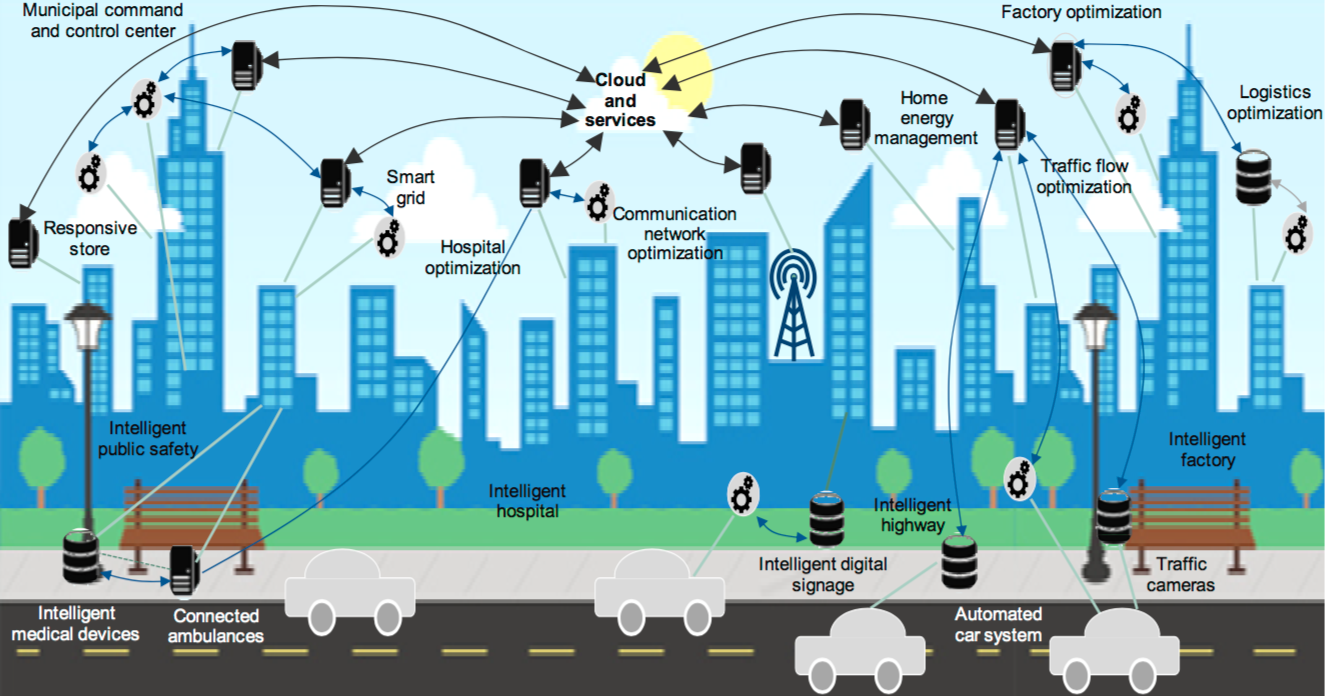
\includegraphics[width=1\textwidth]{Imagens/iotImage.png}
  \caption{Cidade num inv�lucro digital}
  {\bf Fonte:} \cite{CiscoArticle}
  \label{fig:iotImage}
\end{figure}

Na Fig. \ref{fig:iotImage}, organiza��es, pessoas e objetos est�o conectados, criando um inv�lucro digital, composto por representa��es de servi�os conectados a nuvem, tais como: o de um (i) Hospital Inteligente, conectado a dispositivos m�dicos inteligentes e a ambul�ncias; (ii) Centro Digital de Controle e Comando Municipal, integrado a um sistema inteligente de seguran�a p�blica e armazenamento de dados; (iii) Sistema de Otimiza��o de Fluxo de Tr�fico, conectado a um sistema de estradas inteligentes agregadas a c�meras de controle de tr�fico; (iv) F�brica Inteligente, integrada a um sistema de otimiza��o de log�stica e f�brica; (v) Administra��o de Energia Dom�stica e (vi) \textit{Smart Grid} (um novo modelo de Redes El�tricas \cite{IeeeArticle}) e (vii) Otimiza��o de Rede de Comunica��o.

Tais servi�os n�o ser�o estudados nesse trabalho, foram apenas referenciados visando demonstrar uma pequena parte da gama de possibilidades existentes em Cidades Inteligentes, Internet das Coisas, e a problem�tica relacionada ao processamento de dados.

\subsection{Requisitos de uma aplica��o de Cidade Inteligente}

Devido a grande quantidade de dados existentes, conforme mencionado na se��o \ref{iotSection}, a capacidade de processar grandes volumes de dados pode ser um dos requisitos necess�rios a uma aplica��o de Cidade Inteligente. Nesse contexto, por exemplo, pode ser importante observar duas m�tricas: o valor de (i) throughput e  o de (ii) lat�ncia, sendo o primeiro termo referente a taxa de processamento e, o segundo, a varia��o do tempo entre um est�mulo e resposta \cite{WebPerformanceTuning}.

Dependendo dos requisitos da aplica��o, a lat�ncia talvez seja mais interessante de ser priorizada quando respostas a determinados eventos precisam ser no menor intervalo de tempo poss�vel (menos de um segundo). Por outro lado, o valor de throughput, pode ser mais adequado se a aplica��o necessitar processar grandes volumes de dados dentro de um valor de lat�ncia aceit�vel (no m�ximo alguns segundos) \cite{Survey}.

Outro requisito importante de ser analisado, � o de toler�ncia a falhas (necess�rio quando a aplica��o est� inserida em ambientes distribu�dos, ou, de incertezas), o qual permite o funcionamento do sistema mesmo que uma falha (conceito explicado na se��o \ref{realTimePlatforms}) ocorra, o que pode ser obtido, por exemplo, por meio de replica��o \cite{SistemasDistribuidos}. Al�m disso, pode existir a necessidade de antender o requisito de escalabilidade, atrav�s do qual � poss�vel oferecer um servi�o de alta qualidade conforme o aumento da demanda, adicionando novos recursos (escalabilidade horizontal), ou, melhorando os existentes (escalabilidade vertical) \cite{Sommerville}.

Por fim, algumas aplica��es precisam do requisito de Processamento em Tempo Real, quem tem como uma de suas principais caracter�sticas um limite de tempo pr�-determinado para as respostas aos eventos do sistema \cite{Sommerville}. Ap�s mencionar esses requisitos, � importante observar o Modelo de Programa��o (ou, as abstra��es) da plataforma que ser� utilizada no processo de desenvolvimento de uma aplica��o, pois, ele (elas) pode impact�-los.

\subsection{e-Participa��o}

Uma das tem�ticas abordadas em Cidades Inteligentes, � a de promover novos meios para a participa��o do cidad�o nas quest�es relaciondas a gest�o da cidade \cite{AVisionOfSocialMedia}. As Redes Sociais s�o um dos principais meios onde essa intera��o pode ocorrer, posto que elas compostas por um conjunto de pessoas (ou, organiza��es), representando n�s de uma rede, conectadas atrav�s de um conceito abstrato de relacionamento \cite{DccArticle}. 

Sendo assim, tal ambiente virtual, tem proporcionado um novo espa�o para que os cidad�os possam participar de processos de consulta e delibera��o (exame e dicuss�o de um assunto \cite{Priberam}), atuando com os governos como atores de processos de tomadas de decis�o \cite{DccArticle}. Essa participa��o quando ocorre em ambientes virtuais, como Redes Sociais, aplicativos, wiki, f�rum, blogs, dentre outros \cite{AnpocsArticle}, defini-se pelo conceito de e-Participa��o, dentro de outro mais abrangente que � o de Governo Eletr�nico. 

O Governo Eletr�nico � caracterizado pelo uso de TICs pelo governo p�blico, buscando prover melhores servi�os, informa��es e conhecimento ao cidad�o; facitando o acesso ao processo pol�tico e incentivando a participa��o \cite{AnpocsArticle}. Ele pode ser dividido, principalmente, nos tr�s campos seguintes: e-Administra��o, a respeito do funcionamento interno do poder p�blico; e-Governo, no tocante a entrega e fornecimento de servi�os e informa��es qualificadas aos cidad�os; e-Democracia, relacionada a amplia��o da participa��o da sociedade na tomada de decis�o, sendo a e-Participa��o uma sub-�rea desse �ltimo \cite{AnpocsArticle}.

A inten��o da e-Participa��o � refor�ar e renovar as intera��es entre o setor p�blico, os pol�ticos e cidad�os; tanto quanto poss�vel no processo democr�tico \cite{AnpocsArticle}. Al�m disso, a e-Participa��o n�o pode ser avaliada somente por seus aspectos t�cnicos, mas tamb�m quanto a capacidade de incrementar a democracia \cite{AnpocsArticle}.

Um dos desafios nessa �rea � avaliar as ferramentas apoiadas pelas TICs, quanto as formas de engajamento existentes, como informa��o, consulta, ou, participa��o ativa \cite{AnpocsArticle}. Ainda, segundo cita��o contida em \cite{AnpocsArticle}, a e-Participa��o � um conjunto de v�rias tecnologias, medidas sociais e pol�ticas, havendo a necessidade de melhorar a compreens�o das rela��es entre esses componentes e como suas respectivas pr�ticas de avalia��o podem ser aplicadas a e-Particip��o como um todo.

Com isso, para que os processos que a envolvem sejam eficazes � importante considerar os ambientes online e off-line, ou seja, incrementando os m�todos tradicionais (confer�ncias, f�runs, conselhos, ouvidorias, audi�ncias, consultas, reuni�es, comit�s, grupos de trabalho e mesas de negocia��o) com as possibilidades da e-Partici��o, estendendo-a ainda aos grupos desfavorecidos e desconectados \cite{AnpocsArticle}. Dito isso, no par�grafo seguinte, s�o referenciados alguns dos diferentes n�veis de e-Participa��o.   

\paragraph{N�veis de e-Participa��o.} No n�vel e-Informa��o, h� um canal unidirecional, visando apenas fornecer informa��es de interesse c�vico; no de e-Consulta, a comunica��o � biderecional, via coleta de opini�es e alternativas; no de e-Envolvimento busca-se garantir a compreens�o e levar em considera��o os anseios do cidad�o; em e-Colabora��o, a comunica��o � bidirecional, e o cidad�o participa ativamente no desenvolvimento de alternativas e indentifica��o de melhores solu��es; por fim, no de e-Empoderamento, a influ�ncia, controle e elabora��o de pol�ticas pelo e para o p�blico � viabilizada \cite{AnpocsArticle}. 

\section{Plataformas de processamento em tempo real}
\label{realTimePlatforms}

As plataformas de processamento em tempo real \abrv[RTC --� Real� Time Computing]{(RTC, \textit{Real� Time Computing})}, compostas por hardware ou software, s�o sistemas que tem como um dos principais requisitos emitir respostas a eventos de acordo com um determinado \textit{deadline} (limite de tempo). Sendo assim, a corretude da computa��o n�o depende apenas da corretude l�gica, mas tamb�m dos resultados serem produzidos de acordo com o \textit{deadline} especificado \cite{RtcAsNewDiscipline}, \cite{Sommerville}.

Normalmente, os resultados s�o obtidos atrav�s de processamentos realizados por um conjunto de \textit{tasks} (tarefas) cooperativas, iniciadas por eventos do sistema. Os eventos s�o dependentes do ambiente no qual est�o inseridos, podendo ocorrer periodicamente (de forma regular e previs�vel), ou, aperiodicamente (irregulares e imprevis�veis) \cite{RtcAsNewDiscipline}, \cite{Sommerville}.

As \textit{tasks} podem ter uma rela��o de interdepend�ncia e ao mesmo tempo nem todos os eventos que as originaram necessitarem de ser processados dentro de um \textit{deadline}. Apesar disso, nenhuma \textit{task} pode vir a comprometer o processamento de outra \cite{RtcAsNewDiscipline}.  

Com isso, os \textit{deadlines} podem ser classificados em \textit{hard}, \textit{firm}, ou, \textit{soft}. No primeiro caso, respectivamente, as respostas a todos os eventos devem necessariamente ocorrer dentro do  \textit{deadline}  definido; no segundo, \textit{deadlines} esporadicamente n�o atendidos s�o aceitos; no terceiro, \textit{deadlines} n�o alcan�ados s�o permitidos frequentemente \cite{RtcAsNewDiscipline}. Al�m desses categorias, h� os sistemas com \textit{delay} (atraso) introduzido entre o intervalo de tempo de est�mulo e resposta, os quais s�o classificados como \abrv[NRT -- Near Real Time]{\textit{Near Real Time} (NRT)}, ou seja, s�o sistemas de processamento em "quase tempo real".

Sendo assim, na categoria \textit{hard}, � considerado como falha se o tempo estimado para um processamento n�o for atendido, e nas demais, a ocorr�ncia disso resulta numa degrada��o (cont�nua de acordo com a quantidade de \textit{deadlines} n�o atendidos) \cite{RtcAsNewDiscipline}, \cite{Sommerville}. Entende-se por falha quando o usu�rio n�o recebe algo esperado (por exemplo, \textit{deadline} n�o atendido) devido a um erro de sistema. Sendo esse erro um estado err�neo resultante de um defeito (caracter�stica do sistema que pode resultar em erro). E, degrada��o, como decr�scimo da qualidade (conceito subjetivo, de acordo com os requisitos da aplica��o) do sistema \cite{Sommerville}.

Por fim, � importante mencionar tamb�m que uma falha de sistema pode comprometer o requisito de Confian�a e prejudicar um grande n�mero de pessoas \cite{RtcAsNewDiscipline}, \cite{Sommerville}. Na Fig. \ref{fig:reliabilityDiagram} a seguir, s�o ilustradas as principais propriedades desse requisito:

\begin{figure}[htb]
  \centering
    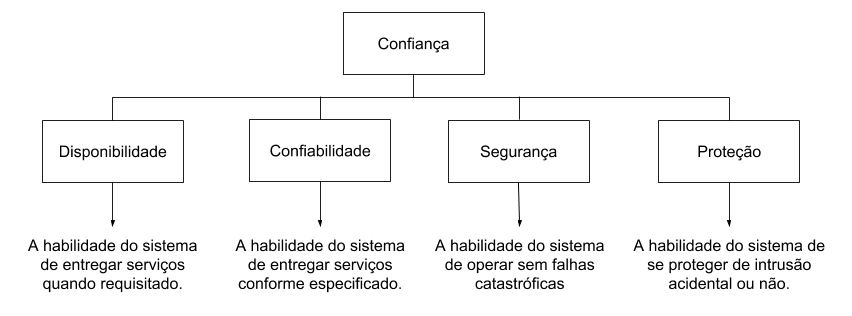
\includegraphics[width=1\textwidth]{Imagens/reliabilityDiagram.png}
  \caption{Principais propriedades de Confian�a}
  {\bf Fonte:} \cite{Sommerville}
  \label{fig:reliabilityDiagram}
\end{figure}

\subsection{Processamento de fluxo de eventos em tempo real}
\label{espSubsection}

Fluxo (ou \textit{stream}) de eventos, basicamente, pode ser entendido como uma s�rie de eventos em fun��o do tempo \cite{Datatorrent}, \cite{Complexevents}. Dentro desse escopo, duas abordagens de processamento s�o importantes diferenciar: \abrv[ESP -- Event Stream Processing]{(i) ESP (\textit{Event Stream Processing}, ou, Processamento de Fluxo de Eventos)} e \abrv[CEP -- Complex Event Processing]{(ii) CEP (\textit{Complex Event Processing}, ou, Processamento Complexo de Eventos)}. A primeira, costuma-se focar principalmente com quest�es de baixo n�vel, relacionadas a como processar eventos em tempo real atendendo requisitos de escalabilidade, toler�ncia a falha, confiabilidade, etc \cite{ConfluentArticle}.

Na segunda abordagem, os \textit{streams} s�o utilizados para criar uma nuvem de eventos, parcialmente ordenados por tempo e causalidade, conceito conhecido como \abrv[POSET -- Partially ordered set of events]{POSET (\textit{Partially Ordered Set of Events})} \cite{Complexevents}. Sendo assim, normalmente, visa-se trabalhar quest�es de alto n�vel, utilizando \textit{posets} para a cria��o de padr�es de eventos, envolvendo seus relacionamentos, estrutura interna, etc. Com esse conjunto de informa��es � poss�vel compor eventos complexos, os quais podem ser consultados continuadamente \cite{ConfluentArticle}. 

Portanto, nessa monografia, ser� utilizada a primeira abordagem (ESP) para processamento de eventos, por ser mais adequada ao objetivo proposto no Cap. \ref{objective}. Em ESPs, algumas plataformas processam os \textit{streams} continuadamente conforme s�o recebidos pelo sistema; paradigma conhecido como \textit{One at Time}. Quando um evento � processado com sucesso, h� a possibilidade de emitir uma notifica��o sobre isso, a qual � custosa devido ao fato de ser necess�rio rastre�-lo at� o t�rmino de seu processamento \cite{Datatorrent}. 

Outra alternativa, � a de realizar o processamento em \textit{micro-batchs} (pequenos lotes) de eventos, tendo com uma das vantagens poder realizar opera��es em pequenos blocos de dados, em vez de individualmente, ao custo de introduzir um pequeno atraso no processo \cite{Datatorrent}.

\section{Apache Spark}
\label{sparkSection}

Apache Spark � uma plataforma de computa��o em \textit{cluster} (unidade l�gica composta por um conjunto de computadores conectados entre si atrav�s da Rede, permitindo compartilhamento de recursos), com suporte a consultas a banco de dados, processamento de streaming (em \textit{Near Real Time}), grafos, e aprendizado de m�quina. Tendo Java, Python e Scala como linguagens de programa��o suportadas \cite{Spark}.

A arquitetura do Spark, conforme a Fig. \ref{fig:sparkStack}, � composta por uma pilha integrando os seguintes componentes, a serem explicados posteriormente: Spark SQL, Spark Streaming, MLib, GraphX, Spark Core e Administradores de Cluster (Yarn \cite{Yarn} e Apache Mesos \cite{Mesos}). Tal estrutura, visa ser de f�cil manuten��o, teste, \textit{deploy}, e permitir aumento de perfomance do n�cleo impactando seus demais componentes.

\begin{figure}[htb]
  \centering
    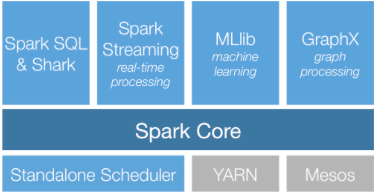
\includegraphics[width=0.5\textwidth]{Imagens/sparkStackImage.png}
  \caption{Ilustra��o da arquitetura em pilha do Apache Spark}
  {\bf Fonte:} \cite{LearningSpark}
  \label{fig:sparkStack}
\end{figure}

\subsection{M�dulos do Apache Spark}

O Spark Core � o principal m�dulo do Apache Spark, respons�vel principalmente pelo gerenciamento de mem�ria,  \textit{tasks} (conceito explicado em \ref{taskSection}) e toler�ncia a falha. Ainda nele, a abstra��o conhecida como  RDD (\textit{Resilient Distributed Datasets}) � definida, cujo papel � o de representar uma cole��o de dados distribu�dos e manipulados em paralelo. Os RDDs em Java s�o representados pela classe JavaRDD, criados atrav�s da classe JavaSparkContext (contexto da aplica��o), que � instanciada recebendo como par�metro um objeto SparkConf, contendo informa��es relacionadas ao nome da aplica��o e o endere�o em que ela ser� executada, pondendo ser local, ou, em cluster.

Outro m�dulo � o Spark Streaming, o qual realiza o processamento de dados em \textit{stream}. Os \textit{streams} s�o representados por uma sequ�ncia de RDDs, conhecida como DStream. O contexto de um \textit{streaming} (JavaStreamingContext) � criado usando as configura��es da aplica��o e o intervalo no qual cada DStream ser� definido. Ap�s isso, tais \textit{streams} s�o atribu�dos a um objeto da classe JavaReceiverInputDStream.

Al�m dos m�dulos detalhados nos par�grafos anteriores, � relevante mencionar o (i) Spark SQL, respons�vel por trabalhar com dados estruturados E consultas SQL; o (ii) MLib, relacionado ao aprendizado de m�quina, contendo algor�timos tais como o de classifica��o, regress�o, "clusteriza��o", filtragem colaborativa, avalia��o de modelo e importa��o de dados; e o (ii) GraphX, que � composto por uma biblioteca para manipula��o de grafos e computa��es paralelas. Por fim, o Spark tamb�m possui um administrador de \textit{cluster} padr�o, conhecido como \textit{Standalone Scheduler} \cite{Spark}, tendo tamb�m suporte ao YARN e Apache Mesos.

\subsection{Composi��o Interna do Apache Spark}
\label{sparkInternalsSection}

Nesta se��o � explicada a composi��o interna do Apache Spark, expondo os componentes que permitem a execu��o distribu�da de uma aplica��o spark, tais como o Driver Program, Spark Context, Worker Node e Executor. Tamb�m, s�o explicados os conceitos sobre as opera��es de Transforma��o e A��o, e os relativos a \textit{Job}, \textit{Stage}, \textit{Task} e Parti��o RDD.

\subsubsection{Modelo de execu��o das aplica��es Spark}
\label{sparkModelSection}

O modelo de execu��o das aplica��es Spark � definido pela rela��o composta por um \textit{driver}, SparkContext, executors e \textit{tasks}, conforme ilustrado na Fig. \ref{fig:sparkComponents}. Nessa intera��o, as aplica��es Spark funcionam num \textit{Worker Node} (qualquer n� capaz de de executar c�digo de aplica��o localmente ou num \textit{cluster}) como uma esp�cie de \textit{Driver}, o qual executa opera��es paralelas e define dados distribu�dos sobre um \textit{cluster}. Al�m disso, o \textit{driver} � respons�vel por encapsular a fun��o principal da aplica��o e prover acesso ao Spark, utilizando o objeto da classe SparkContext. Tal objeto, � usado tamb�m para representar uma conex�o com um \textit{cluster} e construir RDDs \cite{LearningSpark}. 

Ap�s a constru��o de um RDD, � poss�vel executar opera��es sobre ele. Essas opera��es s�o realizadas por \textit{executors}, processos administrados por uma aplica��o Spark (cada aplica��o tem os seus pr�prios \textit{executors}); nos quais h� espa�os reservados para execu��o de \textit{tasks} (conceito explicado na se��o \ref{taskSection}). H� dois tipos de opera��es: (i) A��es (\textit{actions}) e (ii) Transforma��es (\textit{transformations}) \cite{Spark}. O primeiro tipo retorna um resultado ao \textit{driver} ap�s computa��es sob um conjunto de dados, de acordo com uma fun��o. Sendo o segundo, respons�vel por gerar novos conjuntos de dados (RDDs) atrav�s, tamb�m, de fun��es especificadas \cite{LearningSpark}. 

\begin{figure}[htb]
  \centering
    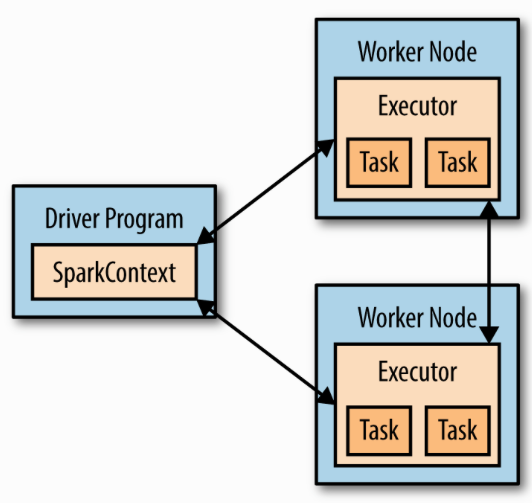
\includegraphics[width=0.5\textwidth]{Imagens/sparkComponentsImage.png}
  \caption{Componentes do Spark para execu��o distribu�da}
  {\bf Fonte:} \cite{LearningSpark}
  \label{fig:sparkComponents}
\end{figure}

\subsubsection{Job}
\label{jobSection}

A abstra��o do conceito de \textit{job} est� relacionada com o de \textit{action}. Mais especificamente, um \textit{job} � o conjunto de est�gios (\textit{stages}) resultantes de uma determinada \textit{action}. Por exemplo, quando o m�todo count() � invocado (para realizar a contagem de elementos dentro de um RDD), cria�-se um \textit{job} composto por um ou mais \textit{stages}. Os \textit{jobs}, por padr�o, s�o escalonados para serem executados em ordem \abrv[FIFO -- First In, First Out]{FIFO (\textit{First In, First Out})}. Al�m disso, o \textit{scheduler} do Spark � respons�vel por criar um plano de execu��o f�sica, o qual � utilizado para calcular as RDDs necess�rias para executar a a��o invocada \cite{LearningSpark}, \cite{SparkInternals}.

Em tal plano de execu��o f�sica, defini�-se basicamente um grafo ac�clico dirigido (DAG), relacionando as depend�ncias existentes entre os RDDs, numa esp�cie de linhagem de execu��o (\textit{lineage}). Ap�s isso, a partir da �ltima RDD do �ltimo est�gio, cada depend�ncia � calculada, de tr�s para frente, para que posteriormente os RDDs dependentes possam ser calculados, at� que todas as \textit{actions} necess�rias tenham terminado \cite{LearningSpark}, \cite{SparkInternals}.

\subsubsection{Stage}
\label{stageSection}

A divis�o de um \textit{job} resulta no conceito de \textit{stage}, ou seja, \textit{jobs} s�o compostos por um ou mais \textit{stages}, os quais t�m  \textit{tasks} a serem executadas. Nem sempre a rela��o entre  stages e RDDs ser� de 1:1. No mais simples dos casos, para cada RDD h� um \textit{stage}, sendo poss�vel nos mais complexos haver mais de um \textit{stage} gerado por um �nico RDD \cite{LearningSpark}, \cite{SparkInternals}.

Por exemplo, havendo tr�s RDDs no grafo RDD, n�o necessariamente haver�o tr�s \textit{stages}. Um dos motivos para isso acontecer � quando ocorre \textit{pipelining}, situa��o na qual � poss�vel reduzir o n�mero de  \textit{stages}, calculando os valores de alguns  RDDs  utilizando unicamente informa��es de seus antecessores, sem movimenta��o de dados de outros RDDs \cite{LearningSpark}, \cite{SparkInternals}.

Al�m da possibilidade do n�mero de \textit{stages} ser reduzido, o contr�rio acontece quando fronteiras entre  \textit{stages} s�o definidas. Tal situa��o, ocorre porque algumas transforma��es, como a reduceByKey (fun��o de agrega��o por chaves), podem resultar em reparticionamento do conjunto de dados para a computa��o de alguma sa�da, exigindo dados de outros RDDs para a forma��o de um �nico RDD. Assim, em cada fronteira entre os \textit{stages}, \textit{tasks} do est�gio antecessor s�o respons�veis por escrever dados para o disco e buscar \textit{tasks} no est�gio sucessor, atrav�s da rede, resultando em um processo custoso, conhecido como shuffling \cite{LearningSpark}, \cite{SparkInternals}.

O n�mero de parti��es entre o est�gio predecessor e sucessor pode ser diferente, sendo poss�vel customiz�-lo, embora isso n�o seja recomend�vel. Tal aconselhamento � devido ao fato de que se o n�mero for modificado para uma pequena quantidade de parti��es, tais podem sofrer com \textit{overloaded tasks}  (sobrecarregadas), do contr�rio, havendo parti��es em excesso, resultar� em um alto n�mero de \textit{shuffling} entre elas \cite{LearningSpark}, \cite{SparkInternals}.

Em resumo, \textit{shuffling} sempre acontecer� quando for necess�rio obter dados de outras parti��es para computar um resultado, sendo esse um procedimento custoso devido ao n�mero de opera��es de entrada e sa�da envolvendo: leitura/escrita em disco e transfer�ncia de dados atrav�s da rede. No entanto, se necess�rio, o Spark prov� uma forma eficiente para reparticionamento, conhecida como coalesce(), a qual reduz o n�mero de parti��es sem causar movimenta��o de dados \cite{LearningSpark}.

\subsubsection{Task}
\label{taskSection}

A abstra��o do conceito \textit{task} est� relacionada principalmente com \textit{stage}, pois, uma vez que os est�gios s�o definidos, \textit{tasks} s�o criadas e enviadas para um \textit{scheduler} interno. Al�m disso, \textit{tasks} est�o muito pr�ximas da defini��o de partition, pelo fato de ser necess�ria a exist�ncia de uma task para cada partition, para executar as computa��es necess�rias sobre ela \cite{LearningSpark}.

Portanto, o n�mero de \textit{tasks} em um stage � definido pelo n�mero de parti��es existentes no RDD antecessor. E, por outro lado, o n�mero de parti��es em um determinado RDD � igual ao n�mero de parti��es existentes no RDD do qual ele depende. No entanto, h� exce��es em caso de (i) \textit{coalescing}, processo o qual permite criar um RDD com menos parti��es que seu antecessor; (ii) uni�o, sendo o n�mero de parti��es resultado da soma do n�mero de parti��es predecessoras; (iii) produto cartesiano, produto dos predecessores \cite{LearningSpark}.

Cada \textit{task} internamente � divida em algumas etapas, sendo elas: (i) carregamento dos dados de entrada, sejam eles provenientes de unidades de armazenamento (caso o RDD seja um RDD de entrada de dados), de um RDD existente (armazenado em mem�ria cache), ou, de sa�das de outro RDD (processo de \textit{shuffling}), (ii) processamento da opera��o necess�ria para computa��o do RDD representado por ela, (iii) escrever a sa�da para o processo de \textit{shuffling}, para um armazenamento externo ou para o \textit{driver} (caso seja o RDD final de uma a��o). Em resumo, uma  textit{task} � respons�vel por coletar os dados de entrada, process�-�los e, por fim, gerar uma sa�da \cite{LearningSpark}.

\section{Apache Storm}
\label{stormSection}

Apache Storm \cite{Storm} � uma plataforma de computa��o em \textit{cluster}, com suporte a processamento de \textit{stream}  de dados em tempo real. O Storm requer pouca manuten��o, � de f�cil de administra��o e tem suporte a qualquer linguagem de programa��o (que leia e escreva fluxos de dados padronizados), posto que em seu n�cleo � utilizado o Apache Thrift \cite{Thrift} (framework que permite o desenvolvimento de servi�os multilinguagem) para definir e submeter topologias (conceito definido em \ref{topologySection}) \cite{Storm}.

A arquitetura do Storm, conforme a Fig. \ref{fig:stormComponents}, � composta pelos seguintes componentes, a serem explicados posteriormente: Nimbus, ZooKeeper e Supervisor Node.

\begin{figure}[htb]
  \centering
    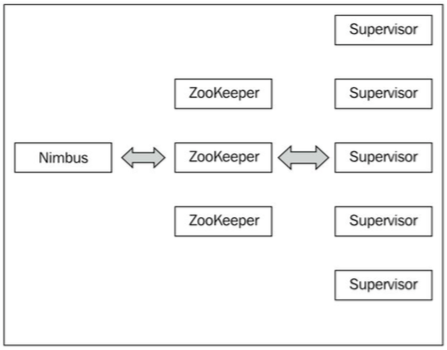
\includegraphics[width=0.5\textwidth]{Imagens/stormComponentsImage.png}
  \caption{Ilustra��o da arquitetura do Apache Storm}
  {\bf Fonte:} \cite{LearningStorm}
  \label{fig:stormComponents}
\end{figure}

\subsection{Composi��o interna do Apache Storm}

Nesta se��o � explicada a composi��o interna do Apache Storm, expondo os principais componentes que permitem a execu��o distribu�da de uma topologia Storm, tais como o Nimbus, ZooKeeper e \textit{Supervisor Nodes}.

\subsubsection{Nimbus}
\label{nimbusSection}

Nimbus � o processo \textit{master} executado num \textit{cluster} Storm, tendo ele uma �nica inst�ncia e sendo respons�vel por distribuir o c�digo da aplica��o (\textit{job}) para os n�s \textit{workers} (computadores que comp�em o \textit{cluster}), aos quais s�o atribu�das \textit{tasks} (parte de um \textit{job}). As \textit{tasks} s�o monitoradas pelo \textit{Supervisor Node}, sendo reiniciadas em caso de falha e quando requisitado. Ainda, caso um \textit{Supervisor Node} falhe continuadamente, o job � atribu�do para outro n� \textit{worker} \cite{LearningStorm}, \cite{StormPython}. 

O Nimbus utiliza um protocolo de comunica��o sem estado (\textit{Stateless Protocol}), ou seja, cada requisi��o � tratada individualmente, sem rela��o com a anterior, n�o armazenando dados ou estado, sendo assim todos os seus dados s�o armazenados no ZooKeeper (definido em \ref{zookeeperSection}). Al�m disso, ele � projetado para ser \textit{fail�-fast}, ou seja, em caso de falha � rapidamente reiniciado, sem afetar as \textit{tasks} em execu��o nos n�s  \textit{workers} \cite{LearningStorm}, \cite{StormPython}.

\subsubsection{Supervisor Node}
\label{supervisorSection}

Cada \textit{Supervisor Node} � respons�vel pela administra��o de um determinado n� do \textit{cluster} Storm; gerenciando o ciclo de vida de processos \textit{workers} relacionados a execu��o das \textit{tasks} (partes de uma topologia) atribu�das a ele pr�prio. Os workers quando em execu��o emitem "sinais de vida" (\textit{heartbeats}), possibilitando o \textit{supervisor} detectar e reiniciar caso n�o estejam respondendo. E, assim como o Nimbus, um \textit{Supervisor Node} � projetado para ser  \textit{fail�-fast} \cite{LearningStorm}, \cite{StormPython}.

\subsubsection{ZooKeeper}
\label{zookeeperSection}

O ZooKeeper Cluster \cite{ZooKeeper} � respons�vel por coordenar processos, informa��es compartilhadas, \textit{tasks} submetidas ao Storm e estados associados ao \textit{cluster}, num contexto distribu�do e de forma confi�vel, sendo poss�vel aumentar o n�vel de confiabilidade tendo mais de um servidor ZooKeeper. O ZooKeeper atua tamb�m como o intermedi�rio da comunica��o entre Nimbus e os \textit{Supervisor Nodes}, pois eles n�o se comunicam diretamente entre si, ambos tamb�m podem ser finalizados sem afetar o \textit{cluster}, visto que todos os seus dados, s�o armazenados no ZooKeeper, como j� mencionado anteriormente \cite{LearningStorm}, \cite{StormPython}.

\subsubsection{Topologia}
\label{topologySection}

A topologia Storm, ilustrada na Fig. \ref{fig:stormTopology}, � uma abstra��o que define um grafo ac�clico dirigido (DAG), utilizado para computa��es de \textit{streams}. Cada n� desse grafo � respons�vel por executar algum processamento, enviando seu resultado para o pr�ximo n� do fluxo. Ap�s definida a topologia, ela pode ser executada localmente ou submetida a um \textit{cluster} \cite{LearningStorm}, \cite{StormPython}.

\textit{Stream} � um dos componentes da topologia Storm, definido como uma sequ�ncia de tuplas independentes e imut�veis, fornecidas por um ou mais \textit{spout} e processadas por um ou mais \textit{bolt}. Cada \textit{stream} tem o seu respectivo ID, que � utilizado pelos \textit{bolts} para consumirem e produzirem as tuplas. As tuplas comp�em uma unidade b�sica de dados, suportando os tipos de dados (serializ�veis) no qual a topologia est� sendo desenvolvida.

\begin{figure}[htb]
  \centering
    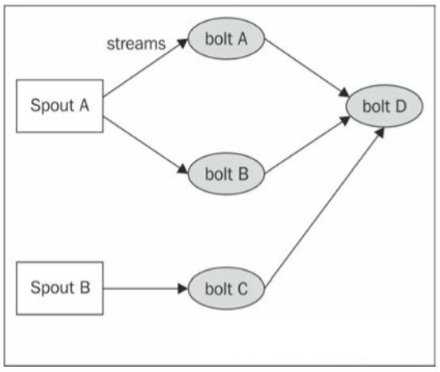
\includegraphics[width=0.5\textwidth]{Imagens/stormTopologyImage.png}
  \caption{Ilustra��o de uma topologia do Storm}
  {\bf Fonte:} \cite{LearningStorm}
  \label{fig:stormTopology}
\end{figure}

\paragraph{Bolt.} Os \textit{bolts} s�o unidades de processamento de dados (\textit{streams}), sendo eles respons�veis por executar transforma��es simples sobre as tuplas, as quais s�o combinadas com outras formando complexas transforma��es. Tamb�m, eles podem ser inscritos para receberem informa��es tanto de outros \textit{bolts}, quanto dos \textit{spouts}, al�m de produzirem \textit{streams} como sa�da \cite{LearningStorm}.

Tais \textit{streams} s�o declarados, emitidos para outro \textit{bolt} e processados, respectivamente, pelos m�todos declareStream, emit e execute. As tuplas n�o precisam ser processadas imediatamente quando chegam a um \textit{bolt}, pois, talvez haja a necessidade de aguardar para executar alguma opera��o de jun��o (\textit{join}) com outra tupla, por exemplo. Tamb�m, in�meros m�todos definidos pela interface Tuple podem recuperar meta�dados associados com a tupla recebida via execute \cite{LearningStorm}.

Por exemplo, se um ID de mensagem est� associado com uma tupla, o m�todo execute dever� publicar um evento \textit{ack}, ou, \textit{fail}, para o \textit{bolt}, caso contr�rio o Storm n�o tem como saber se uma tupla foi processada. Sendo assim, o \textit{bolt} envia automaticamente uma mensagem de confirma��o ap�s o t�rmino da execu��o do m�todo execute e, em caso de um evento de falha, � lan�ada uma exce��o \cite{LearningStorm}.

Al�m disso, num contexto distribu�do, a topologia pode ser serializada e submetida, via Nimbus, para um \textit{cluster}. No qual, ser� processada por \textit{worker nodes}. Nesse contexto, o m�todo prepare pode ser utilizado para assegurar que o \textit{bolt} est�, ap�s a desserializa��o, configurado corretamente para executar as tuplas \cite{LearningStorm}, \cite{StormPython}.

\paragraph{Spout.} Na topologia Storm um \textit{Spout} � o respons�vel pelo fornecimento de tuplas, as quais s�o lidas e escritas por ele utilizando uma fonte externa de dados \cite{LearningStorm}. 

As tuplas emitidas por um  \textit{spout} s�o rastreadas pelo Storm at� terminarem o processamento, sendo emitida uma confirma��o ao t�rmino dele. Tal procedimento somente ocorre se um ID de mensagem foi gerado na emiss�o da tupla e, caso esse ID tenha sido definido como nulo, o rastreamento n�o ir� acontecer \cite{LearningStorm}.

Outra op��o � definir um \textit{time�out} a topologia, sendo dessa forma enviada uma mensagem de falha para o  \textit{spout},  caso a tupla n�o seja processada dentro do tempo estipulado. Sendo necess�rio, novamente, definir um ID de mensagem. O custo dessa confirma��o do processamento ter sido executado com sucesso � a pequena perda de \textit{performance}, que pode ser relevante em determinados contextos; devido a isso � poss�vel ignorar a emiss�o de IDs de mensagens
\cite{LearningStorm}.

Os principais m�todos de um \textit{spout} s�o: o open(), executado quando o \textit{spout} � inicializado, sendo nele definida a l�gica para acesso a dados de fontes externas; o de declara��o de \textit{stream} (declareStream) e o de processamento de pr�xima tupla (nextTuple), que ocorre se houver confirma��o de sucesso da tupla anterior (ack), sendo o m�todo fail chamado pelo Storm caso isso n�o ocorra \cite{LearningStorm}.

Por fim, nenhum dos m�todos utilizados para a constru��o de um  \textit{spout} devem ser bloqueantes, pois o Storm executa todos os m�todos numa mesma \textit{thread}. Al�m disso, todo  \textit{spout} tem um \textit{buffer} interno para o rastreamento dos status das tuplas emitidas, as quais s�o mantidas nele at� uma confirma��o de processamento conclu�do com sucesso (ack) ou falha (fail); n�o sendo inseridas novas tuplas (via nextTuple) no \textit{buffer} quando ele es� cheio \cite{LearningStorm}.

\section{Processamento de Linguagem Natural}

O Processamento de Linguagem Natural (NPL, \textit{Natural Processing Language}) pode ser definido como uma sequ�ncia de computa��es, divididas em est�gios, objetivando entender o significado de determinado texto.  Tal atividade � demasiadamente complexa, por ser dependente do conjunto de caracteres (\textit{charsets}) sendo processados (relacionados com o idioma), do sistema de escrita, do dom�nio da aplica��o, etc \cite{NplBook}. Devido a essa complexidade, a metodologia cl�ssica se divide normalmente nas seguintes fases (ilustradas na Fig. \ref{fig:nlpStages}): \textit{Tokenization}, \textit{Lexical analysis}, \textit{Syntactic analysis}, \textit{Semantic analysis} e \textit{Pragmatic analysis} \cite{NplBook}.

Na fase \textit{Tokenization}, ocorre a extra��o das palavras que comp�em o texto, realizada atrav�s da indentifica��o dos espa�os existentes entre cada palavra. Nos idiomas derivados do Latim, como no caso do Portugu�s, tal estrat�gia pode ser aplicada, pois o sistema de escrita separa as palavras utilizando espa�os entre elas (\textit{space-delimited}), sendo abordadas outras t�cnicas de extra��o para as linguagens n�o segmentadas \cite{NplBook}. Ainda nessa fase, ocorre a segmenta��o do texto, ou seja, a divis�o dos per�odos existentes, na qual precisam ser consideradas quest�es relacionadas a presen�a de pontua��es e s�mbolos \cite{NplBook}.

Em \textit{Lexical analysis}, uma das atividades � a de relacionar varia��es morfol�gicas de uma palavra com seu respectivo lema (a forma mais abstrata de uma palavra, sem flex�es de g�nero, deriva��es, etc) \cite{NplBook}. Sendo assim � poss�vel reduzir a quantidade de palavras em processamento, criar \textit{parsers} (conversores) entre morfologias e lemas, e vice-versa \cite{NplBook}.

Continuando, a fase seguinte � a \textit{Syntactic analysis}, respons�vel pela descri��o estrutural das palavras de acordo com uma gram�tica formal \cite{NplBook}. Um dos conceitos que se pode atribuir a esse est�gio � o de \abrv[POS -- Part-of-speeach]{POS,\textit{Part-of-speeach}}, no qual s�o atribu�das as classes gram�ticais (verbo, adjetivo, artigo, pronome, nome, etc.) de cada palavra, considerando para isso quest�es relacionadas a ambiguidades, contexto a palavra est� inserida, etc. \cite{SmartCityInitiative}, \cite{NplBook}. 

Ao final do est�gio anteriormente mencionado, os resultados dele s�o utilizadas na fase \textit{Semantic analysis}. Nela, as palavras s�o analisadas buscando entender seus respectivos significados, corrigir express�es, senten�as, levando em considera��o o contexto no qual est�o inseridas \cite{NplBook}. Sendo assim, s�o realizadas tradu��es para uma meta-linguagagem, objetivando viabilizar essas analizes \cite{NplBook}. Por fim, o est�gio \textit{Pragmatic analysis}, encontra-se como o �ltimo do fluxo de Processamento de Linguagem Natural, no qual acontece a an�lise das poss�veis inten��es expressas numa senten�a \cite{NplBook}. 


\begin{figure}[htb]
  \centering
    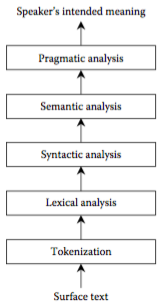
\includegraphics[width=0.3\textwidth]{Imagens/pnl.png}
  \caption{Est�gios de um Processamento de Linguagem Natural}
  {\bf Fonte:} \cite{NplBook}
  \label{fig:nlpStages}
\end{figure}

\section{Aplica��es Web}
	
	% Capitulo 3: Terceiro cap�tulo (arquivo Includes/Capitulo3.tex)
	% Cap�tulo 3
\chapter{Definica��o e execu��o do estudo de caso}
\label{chapter3}

\section{Metodologia de escolha das plataformas para processamento de fluxo de eventos em tempo real}
\label{metodologyOfChoice}

Inicialmente, foi realizada uma pesquisa com a palavra chave "stream processing" e analisados os primeiros artigos (na ordem do resultado e que citavam mais de uma ferramenta) em busca de cita��es a ferramentas (open source) de processamento de streams em tempo real. Com base nesse resultado, os nomes das plataformas encontradas foram utilizados para buscar a quantidade de refer�ncias no Google Scholar (site para publica��o de artigos acad�micos) e Stack Over Flow (site para discuss�o de assuntos relacionados a desenvolvimento de software). Na Tab. \ref{tab:tableNumberOfMentions}, constam os resultados desse procedimento.

A plataforma Esper mencionada em \cite{InfoQArticle} e \cite{ConfluentArticle}. foi descartada do processo de escolha por ser um componente para CEP, normalmente integrado a ferramentas ESPs, fugindo do escopo desse trabalho \cite{EsperTech}. Sendo assim, continuando a an�lise, foram tamb�m consideradas as caracter�sticas das op��es restantes, estudadas superficialmente nos par�grafos seguintes.

\begin{table}[!htb]	
	\center
	{
		\begin{tabular}{c|c|c|c|c}
			\hline
            {\bf Refer�ncia} & {\bf Spark Streaming} & {\bf Storm} & {\bf Flink} & {\bf Samza}\\
			\hline
			\cite{InfoQArticle} & 1 & 1 & 1 & 1\\
			\cite{ConfluentArticle} & 1 & 0 & 0 & 1\\
			\cite{DzoneArticle} & 1 & 1 & 0 & 1\\
			\cite{Datatorrent} & 1 & 1 & 0 & 0\\
			\cite{CakeSolutionsArticle} & 1 & 1 & 0 & 0\\			
			\cite{VenturebeatArticle} & 1 & 1 & 0 & 0\\
			\cite{BravenewgeekArticle} & 1 & 0 & 0 & 1\\
			\cite{GoogleScholar} & 806 & 766 & 171 & 283\\
			\cite{StackOverFlow} & 1541 & 538 & 567 & 87\\
			\hline
			{\bf Total de cita��es} & 2354 & 1311 & 739 & 374\\
			\hline
		\end{tabular}
	}
	% T�tulo de tabelas sempre aparecem antes da tabela
	\caption{Quantidade de cita��es a plataformas ESPs por refer�ncia}
	\label{tab:tableNumberOfMentions}
	{Fonte: Elabora��o pr�pria}	
\end{table}

\paragraph{Apache Spark Streaming.} Apache Spark Streaming � uma extens�o do Spark para processamento de stream, em near real time. Al�m disso, o Spark possui outros m�dulos para consultas a banco de dados, grafos, e aprendizado de m�quina \cite{Spark}. O processamento de stream � realizado em micro-batching pelo Spark Streaming (um de seus m�dulos), utilizando uma abstra��o conhecida como \abrv[DStream -- Discretized Stream]{DStream}, a qual � composta por uma sequ�ncias de \abrv[RDD -- Resilient Distributed Dataset]{RDDs (Resilient Distributed Dataset)}, ilustrada na Fig. \ref{fig:dstream}. RDDs abstraem uma cole��o de dados distribu�dos e manipulados em paralelo. No Spark, tamb�m � poss�vel utilizar processamento em batch, independente do m�dulo que est� sendo utilizado \cite{LearningSpark}.

\begin{figure}[htb]
  \centering
    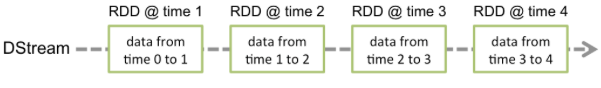
\includegraphics[width=0.8\textwidth]{Imagens/dstreamImage.png}
  \caption{Ilustra��o de um DStream}
  {Fonte:} \cite{Spark}
  \label{fig:dstream}
\end{figure}

\paragraph{Apache Flink.} Apache Flink � um plataforma muito semelhante ao Spark. Com suporte a processamento de streams, os quais s�o definidos por uma abstra��o conhecida como DataStream, ilustrada na Fig. \ref{fig:flinkProcessingImage}. O processamento em batch � realizado em cima de DataSets, semalhantes as RDDs do Spak. Da mesma forma como o DStream � definido como uma s�rie de RDDS, o DataStream � composto por uma sequ�ncia de DataSets. A abstra��o Sink � utilizada para armazenar e retornar DataSets. H� suporte tamb�m para CEP, processamento em grafos, aprendizado de m�quina e consulta a banco de dados \cite{Flink}.

\begin{figure}[htb]
  \centering
    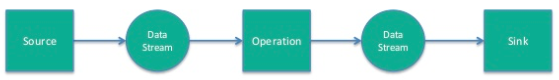
\includegraphics[width=0.8\textwidth]{Imagens/flinkProcessingImage.png}
  \caption{Ilustra��o de um fluxo de processamento no Flink}
  {Fonte:} \cite{FlinkOverView}
  \label{fig:flinkProcessingImage}
\end{figure}

\paragraph{Apache Storm.} Apache Storm � um plataforma para processamento de stream em tempo real. Ao contr�rio do Spark, tem "one at time" como modelo de processamento de dados. As streams s�o compostas por tuplas (unidade b�sica de dados, as quais processadas numa abstra��o conhecida como Topologia, ilustrada na Fig. \ref{fig:stormTopology}, composta por um \abrv[DAG -- Directed Acyclic Graph]{DAG (Directed Acyclic Graph \cite{GraphTeory})} de spouts e bolts, respectivamente, respos�veis por emitir streams de dados e process�-los \cite{LearningStorm}. 

\paragraph{Apache Samza.} Apache Samza � outra plataforma para processamento de stream em tempo real, utilizando como abstra��o base o conceito de mensagem (identificadas por offsets, ids), em vez de tupla, ou, DStream. Os streams s�o separados em parti��es contendo mensagens ordenadas (acessadas apenas no modo de leitura), sendo processados por jobs respons�veis por ler e emir fluxos. Assim como o Spark, h� suporte para processamento em batch, o qual � realizado processando sequ�ncias de streams.

\begin{figure}[htb]
  \centering
    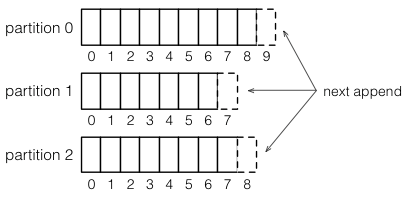
\includegraphics[width=0.6\textwidth]{Imagens/samzaPartitionsImage.png}
  \caption{Ilustra��o de um stream particionado no Samza}
  {Fonte:} \cite{Samza}
  \label{fig:samzaPartitions}
\end{figure}

Ap�s essas breves descri��es das plataformas para processamento de eventos em tempo real e da an�lise realizada do n�mero de cita��es, o Spark Streaming e Storm foram escolhidas como ferramentas para o trabalho desenvolvido no Cap. \ref{chapter3}. Isso, porque ambas possuem maior n�mero de cita��es nas fontes pesquisadas, e consequentemente, comunidades maiores, o que pode favorecer melhor documenta��o, suporte e continuidade desses projetos. 

Sendo assim, como Flink e Samza s�o semelhantes ao Spark o �nico crit�rio de diferencia��o, superfecialmente, � o tamanho da comunidade e a popularidade que o Spark tem. No demais, o Storm se diferencia com o conceito de topologia, interessante de ser estudado. Devido a isso, o Spark e Storm foram aprofundados no Cap. \ref{chapter2} e utilizados no trabalho a ser apresentado nesse cap�tulo.

\section{Aplica��es desenvolvidas para estudo de caso}

Ap�s a escolha das plataformas para processamento de eventos em tempo real, tr�s aplica��es foram desenvolvidas. A primeira, visa processar tweets para coletar m�tricas relacionadas a e-Participa��o; a segunda, processa streams de tweets e realiza processamento de linguagem natural para detectar o sentimento expresso neles; a terceira, exibe numa aplica��o web um mapa contendo as informa��es coletadas nas duas anteriores.

\sloppy
\subsection{Aplica��o para processamento de tweets e coleta de m�tricas relacionadas a e-Participa��o}

O primeiro passo no desenvolvimento dessa aplica��o, foi decidir as contas das quais os tweets seriam processados. Como, normalmente, as capitais dos estados tem maior concentra��o de pessoas, optou-se por fazer um levantamento dos perfis oficiais de suas respectivas prefeituras, para ent�o posteriormente realizar o processamento dos tweets. Sendo assim, a Tab. \ref{tab:tweetAccounts} lista as contas relacionadas as prefeituras municipais das capitais dos vinte e sete estados brasileiros.

Em seguida, foram escolhidas quais m�tricas dessas contas seriam poss�veis e importantes de coletar, tendo como refer�ncia \cite{AVisionOfSocialMedia}. Sendo assim, selecionou-se as seguintes, respectivas ao Twitter: m�dia do n�mero de tweets, seguidores, retweets (compartilhamento de um determinado tweet), coment�rios realizados por usu�rios, r�plicas a tweets e tempo de resposta. As m�tricas referentes ao n�mero de usu�rios acompanhando as listas (jun��es de timelines) do perfil e o total delas existentes foram desconsideras, pois s�o relacionadas a contas diferentes das em quest�o.

De acorco com \cite{AVisionOfSocialMedia}, atrav�s dessas m�tricas � poss�vel obter indicadores relacionados ao n�vel e-Participa��o. Alguns dos indicadores propostos  pela \abrv[SNR -- Social Network Ratio]{SNR (Social Network Ratio)} para Redes Sociais s�o: Atividade, ou, audi�ncia estimada; Tamanho, ou, esfor�o realizado pelo perfil para se comunicar; Visibilidade, ou, n�mero total de men��es ao perfil; Intera��o, ou, capacidade de impacto (viraliza��o) da comunica��o \cite{AVisionOfSocialMedia}.

Portando, pode-se mapear a m�trica m�dia de seguidores ao indicador Atividade, e a de men��es para o de Visibilidade; da mesma forma, as m�dias sobre tweets, r�plicas por dia e tempo de resposta ao indicador Tamanho; por �ltimo, as m�dias de retweets e favoritos ao de Intera��o. A Fig. \ref{fig:twitterDataAnalysisClassDiagram} exibe o diagrama de classes da aplica��o desenvolvida para o processamento de tweets e coleta dessas m�tricas.

\begin{figure}[!htb]
  \centering
    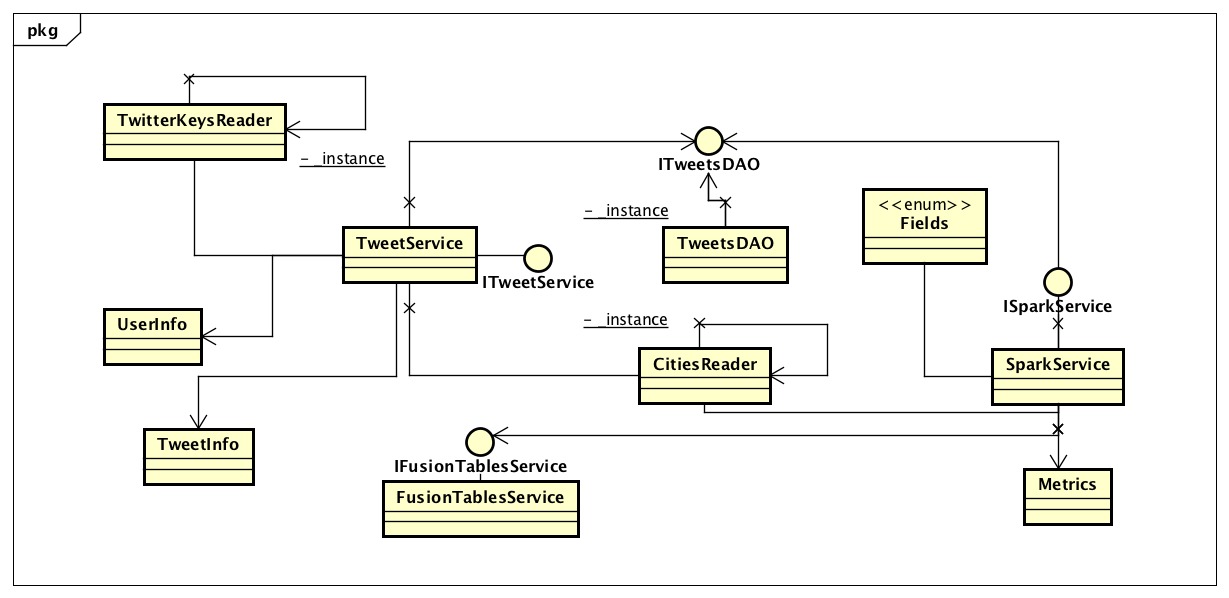
\includegraphics[width=1\textwidth]{Imagens/twitterDataAnalysisClassDiagram.png}
  \caption{Diagrama de classes da aplica��o desenvolvida para processamento e coleta de m�tricas relacionadas a e-Participa��o}
	\begin{flushleft}{Fonte: Elabora��o pr�pria}\end{flushleft}
  \label{fig:twitterDataAnalysisClassDiagram}
\end{figure}

\begin{table}[!htb]	
	\center
	{
		\begin{tabular}{c|c|c}
			\hline
            {\bf Estado} & {\bf Capital} & {\bf Conta no Twitter}\\
			\hline
			Acre & Rio Branco & PrefRioBranco\\
			Alagoas & Macei� & PrefMaceio\\
			Amap� & Macap� & PMMacapa\\
			Amazonas & Manaus & PrefManaus\\
			Bahia & Salvador & agecomsalvador\\			
			Bras�lia & Bras�lia & Gov\_DF\\
			Cear� & Fortaleza & prefeiturapmf\\
			Esp�rito Santo & Vit�ria & VitoriaOnLine\\
			Goi�s & Goi�nia & PrefeituraGy\\
			Maranh�o & S�o Lu�s & PrefeituraSL\\
			Mato Grosso & Cuiab� & prefeitura\_CBA\\
			Mato Grosso do Sul & Campo Grande & cgnoticias\\
			Minas Gerais & Belo Horizonte & prefeiturabh\\
			Paran� & Curitiba & Curitiba\_PMC\\
			Para�ba & Jo�o Pessoa & pmjponline\\
			Par� & Bel�m & prefeiturabelem\\
			Pernambuco & Recife & prefrecife\\
			Piau� & Teresina & prefeitura\_the\\
			Rio Grande do Norte & Natal & NatalPrefeitura\\
			Rio Grande do Sul & Porto Alegre & Prefeitura\_POA\\
			Rio de Janeiro & Rio de Janeiro & Prefeitura\_Rio\\
			Rond�nia & Porto Velho & prefeitura\_pvh\\
			Roraima & Boa Vista & PrefeituraBV\\
			Santa Catarina & Florian�polis & scflorianopolis\\
			Sergipe & Aracaju & PrefeituraAracaju\\
			S�o Paulo & S�o Paulo & prefsp\\
			Tocantins & Palmas & cidadepalmasy\\
			\hline
		\end{tabular}
	}
	% T�tulo de tabelas sempre aparecem antes da tabela
	\caption{Contas do Twitter relacionadas as prefeituras municipais das capitais dos vinte e sete estados brasileiros}
	\label{tab:tweetAccounts}
	\begin{flushleft}{Fonte: Elabora��o pr�pria}\end{flushleft}
\end{table}
 
	
	% Capitulo 4: Quarto cap�tulo (arquivo Includes/Capitulo4.tex)
	% Cap�tulo 4
\chapter{Resultados e Trabalhos Relacionados}

\section{Resultados}

A - tweets por dia
B - retweets por dia
C - favoritos
D - r�plicas
E - tempo de resposta
F - men��es

\sloppy

\begin{table}[!htb]
	\center
		% T�tulo de tabelas sempre aparecem antes da tabela
	\caption{Coloca��o dos perfis das prefeituras das capitais, de acordo com suas respectivas m�tricas}
	\bigskip
	\label{tab:rankMetrics}
	{
		\begin{tabular}{c|c|c|c|c|c|c|c|c|c}
			\hline
            {\bf UF} & {\bf Capital} & {\bf A} & {\bf B} & {\bf C} & {\bf D} & {\bf E} & {\bf F} & {\bf Pontua��o} & {\bf Coloca��o}\\
			\hline
			AC & Rio Branco & 24 & 20 & 23 & 22 & 1 & 19 & 109 & 19\\
			AL & Macei� & 12 & 19 & 17 & 10 & 19 & 18 & 88 & 15\\
			AM & Manaus & 21 & 18 & 16 & 17 & 14 & 22 & 102 & 18\\
			AP & Macap� & 14 & 3 & 6 & 7 & 13 & 12 & 49 & 5\\
			BA & Salvador & 18 & 25 & 25 & 27 & 0 & 27 & 0 & 0\\	
			CE & Fortaleza & 16 & 15 & 13 & 21 & 10 & 9 & 84 & 14\\
			DF & Bras�lia & 10 & 10 & 11 & 18 & 3 & 13 & 65 & 10\\
			ES & Vit�ria & 15 & 23 & 21 & 13 & 8 & 21 & 96 & 16\\
			GO & Goi�nia & 1 & 11 & 12 & 15 & 4 & 4 & 44 & 3\\
			MA & S�o Lu�s & 6 & 1 & 1 & 9 & 11 & 8 & 29 & 1\\
			MG & Belo Horizonte & 19 & 9 & 5 & 12 & 7 & 10 & 57 & 7\\
			MS & Campo Grande & 20 & 26 & 27 & 25 & 5 & 26 & 129 & 22\\
			MT & Cuiab� & 26 & 27 & 24 & 20 & 15 & 23 & 129 & 22\\
			PA & Bel�m & 27 & 22 & 19 & 16 & 16 & 20 & 120 & 21\\		
			PB & Jo�o Pessoa & 2 & 16 & 14 & 4 & 24 & 7 & 59 & 8\\
			PE & Recife & 11 & 14 & 10 & 3 & 25 & 6 & 61 & 9\\
			PI & Teresina & 13 & 6 & 18 & 5 & 17 & 16 & 68 & 12\\
			PR & Curitiba & 8 & 2 & 2 & 1 & 21 & 2 & 29 & 1\\
			RJ & Rio de Janeiro & 17 & 7 & 4 & 14 & 12 & 1 & 48 & 4\\
			RN & Natal & 9 & 8 & 7 & 19 & 6 & 17 & 66 & 11\\
			RR & Boa Vista & 24 & 24 & 22 & 0 & 22 & 24 & 116 & 20\\
			RO & Porto Velho & 23 & 21 & 26 & 26 & 0 & 25 & 0 & 0\\
			RS & Porto Alegre & 3 & 5 & 8 & 6 & 20 & 14 & 49 & 5\\
			SC & Florian�polis & 25 & 17 & 20 & 23 & 9 & 5 & 99 & 17\\
			SE & Aracaju & 7 & 13 & 15 & 24 & 2 & 15 & 76 & 13\\
			SP & S�o Paulo & 5 & 4 & 3 & 2 & 23 & 3 & 32 & 2\\
			TO & Palmas & 4 & 12 & 9 & 8 & 18 & 11 & 55 & 6\\
		\end{tabular}
	}
		\begin{flushleft}{\bf Fonte:} Elabora��o pr�pria\end{flushleft}
\end{table}


\begin{table}[!htb]
	\center
		% T�tulo de tabelas sempre aparecem antes da tabela
	\caption{M�tricas relacionadas ao n�mero de tweets por dia dos perfis das prefeituras das capitais, referentes aos 3.200 tweets anteriores a 18/05/2016}
	\bigskip
	\label{tab:tweetPerDayMetrics}
	{
		\begin{tabular}{c|c|c|c|c|c|c|c}
			\hline
            {\bf UF} & {\bf Capital} & {\bf M�dia} & {\bf Med.} & {\bf M�n.} & {\bf M�x.} & {\bf Vari�ncia} & {\bf D. Padr�o}\\
			\hline
			AC & Rio Branco & 4.1106 & 4 & 1 & 23 & 5.0945 & 2.2571\\
			AL & Macei� & 9.9378 & 10 & 1 & 35 & 15.3750 & 3.9210\\
			AM & Manaus & 6.5040 & 6 & 1 & 44 & 26.4491 & 5.1428\\
			AP & Macap� & 9.0395 & 7 & 1 & 37 & 51.0492 & 7.1448\\			
			BA & Salvador & 7.6875 & 6 & 1 & 36 & 30.0648 & 5.4831\\
			CE & Fortaleza & 8.1012 & 8 & 1 & 24 & 16.4454 & 4.0552\\	
			DF & Bras�lia & 10.0946 & 10 & 1 & 63 & 31.2339 & 5.5887\\			
			ES & Vit�ria & 8.6253 & 8 & 1 & 71 & 33.3448 & 5.7744\\
			GO & Goi�nia & 41.0000 & 39 & 1 & 104 & 684.2307 & 26.1578\\			
			MA & S�o Lu�s & 15.6862 & 14 & 5 & 38 & 18.0192 & 4.2449\\
			MG & Belo Horizonte & 7.5805 & 7 & 1 & 24 & 9.1297 & 3.0215\\
			MS & Campo Grande & 7.2539 & 6 & 1 & 30 & 35.1735 & 5.9307\\			
			MT & Cuiab� & 3.5794 & 3 & 1 & 32 & 6.6888 & 2.5862\\
			PA & Bel�m & 3.5637 & 3 & 1 & 13 & 4.3063 & 2.0751\\
			PB & Jo�o Pessoa & 25.3968 & 27 & 3 & 45 & 110.1917 & 10.4972\\
			PE & Recife & 10.0597 & 9 & 1 & 35 & 40.2259 & 6.3423\\
			PI & Teresina & 9.7530 & 9 & 1 & 32 & 29.1127 & 5.3956\\
			PR & Curitiba & 13.1106 & 11 & 1 & 47 & 87.721 & 9.3659\\
			RJ & Rio de Janeiro & 7.9404 & 7 & 1 & 39 & 29.7185 & 5.4514\\
			RN & Natal & 10.2893 & 10 & 1 & 27 & 30.3406 & 5.5082\\
			RO & Porto Velho & 4.4649 & 4 & 1 & 24 & 6.7806 & 2.6039\\
			RR & Boa Vista & 4.5070 & 4 & 1 & 23 & 8.2865 & 2.8786\\
			RS & Porto Alegre & 22.0689 & 19 & 1 & 126 & 348.9193 & 18.6793\\
			SC & Florian�polis & 3.7037 & 3 & 1 & 25 & 13.9446 & 3.7342\\
			SE & Aracaju & 13.2780 & 15 & 1 & 39 & 76.6737 & 8.7563\\
			SP & S�o Paulo & 17.0159 & 16 & 1 & 61 & 100.1433 & 10.0071\\
			TO & Palmas & 19.0297 & 18 & 2 & 53 & 47.2550 & 6.8742\\
		\end{tabular}
	}
		\begin{flushleft}{\bf Fonte:} Elabora��o pr�pria\end{flushleft}
\end{table}

\begin{table}[!htb]
	\center
		% T�tulo de tabelas sempre aparecem antes da tabela
	\caption{M�tricas relacionadas ao n�mero de retweets dos perfis das prefeituras das capitais, referentes aos 3.200 tweets anteriores a 18/05/2016}
	\bigskip
	\label{tab:retweetsMetrics}
	{
		\begin{tabular}{c|c|c|c|c|c|c|c}
			\hline
            {\bf \abrv[Unidade Federativa -- UF]{UF}} & {\bf Capital} & {\bf M�dia} & {\bf Med.} & {\bf M�n.} & {\bf M�x.} & {\bf Vari�ncia} & {\bf D. Padr�o}\\
			\hline
			AC & Rio Branco & 0.3885 & 0 & 0 & 33 & 1.5863 & 1.2595\\
			AL & Macei� & 0.4881 & 0 & 0 & 49 & 2.0948 & 1.4473\\
			AM & Manaus & 0.4962 & 0 & 0 & 162 & 12.5106 & 3.5370\\
			AP & Macap� & 5.8987 & 5 & 0 & 37 & 21.9878 & 4.6891\\		
			BA & Salvador & 0.0837 & 0 & 0 & 2 & 0.0929 & 0.3049\\
			CE & Fortaleza & 0.7656 & 0 & 0 & 32 & 1.5338 & 1.2384\\		
			DF & Bras�lia & 1.6449 & 1 & 0 & 329 & 63.2714 & 1.9681\\
			ES & Vit�ria & 0.3018 & 0 & 0 & 23 & 0.7576 & 0.8704\\
			GO & Goi�nia & 1.6332 & 1 & 0 & 18 & 3.5193 & 1.8759\\		
			MA & S�o Lu�s & 14.5868 & 15 & 0 & 47 & 147.1399 & 12.1301\\
			MG & Belo Horizonte & 2.5498 & 1 & 0 & 308 & 53.3316 & 7.3028\\
			MS & Campo Grande & 0.0784 & 0 & 0 & 3 & 0.0841 & 0.2901\\
			MT & Cuiab� & 0.0765 & 0 & 0 & 4 & 0.0919 & 0.3032\\			
			PA & Bel�m & 0.3258 & 0 & 0 & 10 & 0.6245 & 0.7902\\
			PB & Jo�o Pessoa & 0.6059 & 0 & 0 & 14 & 1.4487 & 1.2036\\
			PE & Recife & 1.3226 & 0 & 0 & 74 & 12.8881 & 3.5900\\
			PI & Teresina & 2.7886 & 0 & 0 & 2274 & 2822.6661 & 53.1287\\
			PR & Curitiba & 7.9868 & 1 & 0 & 842 & 1044.1073 & 32.3126\\		
			RJ & Rio de Janeiro & 2.6015 & 1 & 0 & 2868 & 2611.8290 & 51.1060\\
			RN & Natal & 2.5653 & 2 & 0 & 45 & 13.9157 & 3.7303\\
			RO & Porto Velho & 0.3559 & 0 & 0 & 5 & 1.0223 & 1.0111\\
			RR & Boa Vista & 0.2621 & 0 & 0 & 20 & 0.9140 & 0.9560\\
			RS & Porto Alegre & 4.9975 & 2 & 0 & 209 & 106.0212 & 10.2966\\	
			SC & Florian�polis & 0.5096 & 0 & 0 & 27 & 1.1811 & 1.0868\\
			SE & Aracaju & 1.3246 & 1 & 0 & 14 & 1.8780 & 1.3704\\
			SP & S�o Paulo & 5.2272 & 3 & 0 & 237 & 104.7239 & 10.2334\\
			TO & Palmas & 1.3872 & 1 & 0 & 31 & 3.3871 & 1.8404\\
		\end{tabular}
	}
		\begin{flushleft}{\bf Fonte:} Elabora��o pr�pria\end{flushleft}
\end{table}

\begin{table}[!htb]
	\center
		% T�tulo de tabelas sempre aparecem antes da tabela
	\caption{M�tricas relacionadas ao n�mero de favoritos dos perfis das prefeituras das capitais, referentes aos 3.200 tweets anteriores a 18/05/2016}
	\bigskip
	\label{tab:favoritesMetrics}
	{
		\begin{tabular}{c|c|c|c|c|c|c|c}
			\hline
            {\bf UF} & {\bf Capital} & {\bf M�dia} & {\bf Med.} & {\bf M�n.} & {\bf M�x.} & {\bf Vari�ncia} & {\bf D. Padr�o}\\
			\hline
			AC & Rio Branco & 0.1981 & 0 & 0 & 10 & 0.2872 & 0.5359\\
			AL & Macei� & 0.8884 & 0 & 0 & 32 & 2.9797 & 1.72618\\
			AM & Manaus & 1.0487 & 1 & 0 & 40 & 3.5744 & 1.8906\\
			AP & Macap� & 3.3284 & 3 & 0 & 22 & 7.8843 & 2.8079\\
			BA & Salvador & 0.0821 & 0 & 0 & 2 & 0.0916 & 0.3027\\	
			CE & Fortaleza & 1.8134 & 1 & 0 & 22 & 2.6636 & 1.6320\\	
			DF & Bras�lia & 1.9681 & 1 & 0 & 504 & 160.0064 & 12.6493\\
			ES & Vit�ria & 0.4421 & 0 & 0 & 15 & 0.6922 & 0.8320\\
			GO & Goi�nia & 1.9177 & 1 & 0 & 20 & 3.7246 & 1.9299\\
			MA & S�o Lu�s & 16.3471 & 18 & 0 & 63 & 149.8610 & 12.2417\\
			MG & Belo Horizonte & 3.4410 & 2 & 0 & 257 & 37.6513 & 6.1360\\
			MS & Campo Grande & 0.0025 & 0 & 0 & 1 & 0.0024 & 0.0499\\			
			MT & Cuiab� & 0.1206 & 0 & 0 & 8 & 0.1629 & 0.4036\\
			PA & Bel�m & 0.5028 & 0 & 0 & 9 & 0.8356 & 0.9141\\
			PB & Jo�o Pessoa & 1.1934 & 1 & 0 & 37 & 4.0453 & 2.0113\\
			PE & Recife & 2.1312 & 1 & 0 & 39 & 8.2941 & 2.8799\\
			PI & Teresina & 0.8487 & 0 & 0 & 12 & 1.5913 & 1.2614\\
			PR & Curitiba & 12.7833 & 1 & 0 & 443 & 698.3285 & 26.4259\\
			RN & Natal & 2.6521 & 2 & 0 & 25 & 7.8230 & 2.7969\\
			RJ & Rio de Janeiro & 3.5790 & 2 & 0 & 2216 & 1543.9374 & 39.2929\\
			RO & Porto Velho & 0.0324 & 0 & 0 & 9 & 0.0934 & 0.3057\\
			RR & Boa Vista & 0.3943 & 0 & 0 & 9 & 0.6482 & 0.8051\\
			RS & Porto Alegre & 2.2115 & 0 & 0 & 117 & 37.0543 & 6.0872\\		
			SC & Florian�polis & 0.4428 & 0 & 0 & 22 & 1.1186 & 1.0576\\
			SE & Aracaju & 1.1550 & 1 & 0 & 10 & 1.9697 & 1.4034\\
			SP & S�o Paulo & 4.3504 & 0 & 0 & 213 & 101.2060 & 10.0601\\
			TO & Palmas & 2.2001 & 1 & 0 & 40 & 7.5964 & 2.7561\\
		\end{tabular}
	}
		\begin{flushleft}{\bf Fonte:} Elabora��o pr�pria\end{flushleft}
\end{table}

\begin{table}[!htb]
	\center
		% T�tulo de tabelas sempre aparecem antes da tabela
	\caption{M�tricas relacionadas ao n�mero de r�plicas dos perfis das prefeituras das capitais, referentes aos 3.200 tweets anteriores a 18/05/2016}
	\bigskip
	\label{tab:inReplyMetrics}
	{
		\begin{tabular}{c|c|c|c|c|c|c|c}
			\hline
            {\bf UF} & {\bf Capital} & {\bf M�dia} & {\bf Med.} & {\bf M�n.} & {\bf M�x.} & {\bf Vari�ncia} & {\bf D. Padr�o}\\
			\hline
			AC & Rio Branco & 0.0046 & 0 & 0 & 1 & 0.0046 & 0.0683\\
			AL & Macei� & 0.0800 & 0 & 0 & 1 & 0.0736 & 0.2712\\		
			AM & Manaus & 0.0228 & 0 & 0 & 1 & 0.0222 & 0.1493\\
			AP & Macap� & 0.0884 & 0 & 0 & 1 & 0.0806 & 0.2839\\
			BA & Salvador & 0 & 0 & 0 & 0 & 0 & 0\\
			CE & Fortaleza & 0.0099 & 0 & 0 & 1 & 0.0098 & 0.0994\\		
			DF & Bras�lia & 0.0218 & 0 & 0 & 1 & 0.0213 & 0.1462\\		
			ES & Vit�ria & 0.0356 & 0 & 0 & 1 & 0.0343 & 0.1853\\
			GO & Goi�nia & 0.0253 & 0 & 0 & 1 & 0.0246 & 0.1571\\
			MA & S�o Lu�s & 0.0825 & 0 & 0 & 1 & 0.0756 & 0.2751\\
			MG & Belo Horizonte & 0.0375 & 0 & 0 & 1 & 0.0361 & 0.1900\\
			MS & Campo Grande & 0.0012 & 0 & 0 & 1 & 0.0012 & 0.0353\\
			MT & Cuiab� & 0.0118 & 0 & 0 & 1 & 0.0117 & 0.1083\\						
			PA & Bel�m & 0.0244 & 0 & 0 & 1 & 0.0238 & 0.1545\\
			PB & Jo�o Pessoa & 0.2106 & 0 & 0 & 1 & 0.1662 & 0.4077\\		
			PE & Recife & 0.2525 & 0 & 0 & 1 & 0.1887 & 0.4344\\
			PI & Teresina & 0.1337 & 0 & 0 & 1 & 0.1158 & 0.3404\\
			PR & Curitiba & 0.5395 & 1 & 0 & 1 & 0.2484 & 0.4984\\			
			RJ & Rio de Janeiro & 0.0315 & 0 & 0 & 1 & 0.0305 & 0.1748\\
			RN & Natal & 0.0118 & 0 & 0 & 1 & 0.0117 & 0.1083\\			
			RO & Porto Velho & 0 & 0 & 0 & 0 & 0 & 0\\
			RR & Boa Vista & 0.0403 & 0 & 0 & 1 & 0.0386 & 0.1966\\
			RS & Porto Alegre & 0.1231 & 0 & 0 & 1 & 0.1079 & 0.3285\\
			SC & Florian�polis & 0.0046 & 0 & 0 & 1 & 0.0046 & 0.0683\\
			SE & Aracaju & 0.0015 & 0 & 0 & 1 & 0.0015 & 0.0394\\
			SP & S�o Paulo & 0.2719 & 0 & 0 & 1 & 0.1979 & 0.4449\\
			TO & Palmas & 0.0878 & 0 & 0 & 1 & 0.0801 & 0.2831\\
		\end{tabular}
	}
		\begin{flushleft}{\bf Fonte:} Elabora��o pr�pria\end{flushleft}
\end{table}

\begin{table}[!htb]
	\center
		% T�tulo de tabelas sempre aparecem antes da tabela
	\caption{M�tricas relacionadas ao tempo de resposta (em minutos) dos perfis das prefeituras das capitais, referentes aos 3.200 tweets anteriores a 18/05/2016}
	\bigskip
	\label{tab:responseTimeMetrics}
	{
		\begin{tabular}{c|c|c|c|c|c|c|c}
			\hline
            {\bf UF} & {\bf Capital} & {\bf M�dia} & {\bf Med.} & {\bf M�n.} & {\bf M�x.} & {\bf Vari�ncia} & {\bf D. Padr�o}\\
			\hline
			AC & Rio Branco & 0.0970 & 0 & 0 & 214 & 14.9066 & 3.8609\\
			AL & Macei� & 47.8646 & 0 & 0 & 4360 & 86593.4688 & 294.2676\\		
			AM & Manaus & 16.3806 & 0 & 0 & 9501 & 64431.6201 & 253.8338\\
			AP & Macap� & 10.5509 & 0 & 0 & 2341 & 12090.3230 & 109.9560\\
			BA & Salvador & 0 & 0 & 0 & 0 & 0 & 0\\	
			CE & Fortaleza & 9.9012 & 0 & 0 & 5039 & 35491.4871 & 188.3918\\
			DF & Bras�lia & 2.0675 & 0 & 0 & 1291 & 1593.4398 & 0.1060\\			
			ES & Vit�ria & 6.7112 & 0 & 0 & 9607 & 35471.7322 & 188.3394\\
			GO & Goi�nia & 2.5384 & 0 & 0 & 1108 & 1688.0865 & 41.0863\\			
			MA & S�o Lu�s & 10.0528 & 0 & 0 & 4334 & 14292.01 & 119.5491\\
			MG & Belo Horizonte & 3.9512 & 0 & 0 & 4522 & 8943.9869 & 94.5726\\
			MS & Campo Grande & 2.7471 & 0 & 0 & 2905 & 7902.8722 & 88.8981\\			
			MT & Cuiab� & 26.1856 & 0 & 0 & 35914 & 540769.2511 & 735.3701\\			
			PA & Bel�m & 27.1967 & 0 & 0 & 5443 & 83814.4537 & 289.5072\\
			PB & Jo�o Pessoa & 352.4075 & 0 & 0 & 27344 & 2726035.1595 & 1651.0709\\
			PE & Recife & 669.4376 & 0 & 0 & 72134 & 13843379.6277 & 3720.6692\\
			PI & Teresina & 29.9327 & 0 & 0 & 4155 & 47570.1533 & 218.1058\\
			PR & Curitiba & 83.9431 & 0 & 0 & 25372 & 1141796.2367 & 1068.5486\\
			RJ & Rio de Janeiro & 10.2378 & 0 & 0 & 7342 & 37814.4137 & 194.4592\\
			RN & Natal & 3.40625 & 0 & 0 & 2752 & 4488.0193 & 66.9926\\
			RO & Porto Velho & 0 & 0 & 0 & 0 & 0 & 0\\
			RR & Boa Vista & 120.8646 & 0 & 0 & 45988 & 2604294.3432 & 1613.7826\\
			RS & Porto Alegre & 52.7303 & 0 & 0 & 11821 & 186125.3069 & 431.4224\\	
			SC & Florian�polis & 6.7381 & 0 & 0 & 3989 & 17523.7701 & 132.3773\\
			SE & Aracaju & 0.8018 & 0 & 0 & 1590 & 913.1263 & 30.2179\\
			SP & S�o Paulo & 240.1481 & 0 & 0 & 11561 & 813833.7904 & 902.1273\\
			TO & Palmas & 33.2355 & 0 & 0 & 52091 & 901583.5269 & 949.5175\\
		\end{tabular}
	}
		\begin{flushleft}{\bf Fonte:} Elabora��o pr�pria\end{flushleft}
\end{table}

\begin{table}[!htb]
	\center
		% T�tulo de tabelas sempre aparecem antes da tabela
	\caption{M�tricas relacionadas ao n�mero de men��es por dia dos perfis das prefeituras das capitais, referentes aos 3.200 tweets anteriores a 18/05/2016}
	\bigskip
	\label{tab:mentionsMetrics}
	{
		\begin{tabular}{c|c|c|c|c|c|c|c}
			\hline
            {\bf UF} & {\bf Capital} & {\bf M�dia} & {\bf Med.} & {\bf M�n.} & {\bf M�x.} & {\bf Vari�ncia} & {\bf D. Padr�o}\\
			\hline
			AC & Rio Branco & 7.7777 & 9 & 2 & 11 & 6.3950 & 2.5288\\
			AL & Macei� & 11.8888 & 6 & 3 & 59 & 286.5432 & 16.9275\\			
			AM & Manaus & 4.1428 & 5 & 2 & 7 & 2.9795 & 1.7261\\
			AP & Macap� & 41.7 & 28 & 3 & 107 & 1210.21 & 34.7880\\
			BA & Salvador & 0 & 0 & 0 & 0 & 0 & 0\\
			CE & Fortaleza & 47.7 & 49 & 67 & 26 & 148.6099 & 12.1905\\	
			DF & Bras�lia & 35.8 & 40 & 16 & 50 & 123.7599 & 11.1247\\			
			ES & Vit�ria & 4.8 & 4 & 1 & 12 & 10.9599 & 3.3105\\
			GO & Goi�nia & 85.4 & 76 & 24 & 154 & 1681.04 & 41\\		
			MA & S�o Lu�s & 51.9 & 56 & 5 & 89 & 459.6899 & 21.4403\\
			MG & Belo Horizonte & 42.3 & 43 & 7 & 66 & 256.81 & 16.0252\\
			MS & Campo Grande & 0 & 0 & 0 & 0 & 0 & 0\\			
			MT & Cuiab� & 1.6666 & 1 & 1 & 3 & 0.5555 & 0.7453\\			
			PA & Bel�m & 7.5555 & 7 & 3 & 13 & 8.2469 & 2.8717\\
			PB & Jo�o Pessoa & 52.8888 & 51 & 28 & 82 & 244.0987 & 15.6236\\
			PE & Recife & 58.3333 & 50 & 42 & 89 & 299.5555 & 17.3076\\
			PI & Teresina & 21.3333 & 18 & 11 & 35 & 67.1111 & 8.1921\\
			PR & Curitiba & 155.4 & 128 & 5 & 250 & 18288.0399 & 135.2332\\
			RJ & Rio de Janeiro & 354 & 208 & 182 & 1550 & 179198.6666 & 423.3186\\
			RN & Natal & 19.875 & 19 & 2 & 37 & 110.8593 & 10.5289\\
			RO & Porto Velho & 0 & 0 & 0 & 0 & 0 & 0\\
			RR & Boa Vista & 0 & 0 & 0 & 0 & 0 & 0\\
			RS & Porto Alegre & 32.8 & 36 & 11 & 44 & 112.56 & 10.6094\\
			SC & Florian�polis & 61.75 & 61 & 36 & 89 & 532.1875 & 23.0691\\
			SE & Aracaju & 22.2 & 18 & 4 & 47 & 175.1599 & 13.2348\\
			SP & S�o Paulo & 113 & 127 & 13 & 196 & 4026.2 & 63.4523\\
			TO & Palmas & 41.7777 & 35 & 27 & 85 & 262.6172 & 16.2054\\
		\end{tabular}
	}
		\begin{flushleft}{\bf Fonte:} Elabora��o pr�pria\end{flushleft}
\end{table}

\section{Trabalhos Relacionados}
	
	% Capitulo 5: Quinto cap�tulo (arquivo Includes/Capitulo5.tex)
	% Cap�tulo 5
\chapter{Conclus�es}
\label{chapter5}

Atualmente, a quantidade de pessoas e coisas conectadas � Internet tem gerado dados massivamente, os quais processados podem ajudar a resolver importantes problemas enfrentados pela sociedade. Por exemplo, como demonstrado nesse trabalho, � poss�vel utilizar ferramentas para processamento de grande volume de dados buscando obter uma vis�o do n�vel de e-Participa��o em Redes Sociais.

Embora indicadores sobre o n�vel de e-Participa��o sejam importantes, alguns estudos t�m classificado determinadas cidades como inteligentes, sem lev�-los em considera��o. O que � um problema, pois os cidad�os podem desempenhar relevantes contribui��es com o governo local, objetivando o desenvolvimento da cidade e resolu��o de problemas ainda existentes. 

Muitas prefeituras do Brasil, principalmente as afastadas das grandes metr�poles, de acordo com as m�tricas coletadas, tem feito pouco uso de seus perfis no Twitter, indicando um baixo n�vel de intera��o entre seus respectivos governos locais e cidad�os. Em contraste, as prefeituras com melhores classifica��es de e-Participa��o, encontram-se pr�ximas as regi�es litor�neas, com maior desenvolvimento econ�mico.

Nos aspectos do desenvolvimento das aplica��es, conclui-se que a ferramenta Spark � a melhor indicada para processamento de \textit{tweets} em \textit{batch}, enquanto que o Storm � mais aconselhado para o processamento de stream de \textit{tweets}, principalmente devido a sua arquitetura de Toler�ncia a Falhas. 

Considerando o exposto nos par�grafos anteriores, os objetivos dessa monografia foram alcan�ados. Sendo assim, esse trabalho contribui com uma aplica��o para processamento em \textit{batch} de \textit{tweets}, capaz de coletar e exibir, atrav�s de uma interface web, m�tricas relacionadas a e-Participa��o. Assim como, processamento de \textit{stream} de \textit{tweets} utilizando diferentes plataformas (indicando a mais adequada aos requisitos da aplica��o), obtendo suas respectivas polaridades de sentimentos, exibidas tamb�m no mapa.

Consequentemente, colaborando com uma vis�o sobre as situa��es das m�tricas relacionadas a e-Participa��o das capitais dos estados brasileiros. Possibilitando que gestores e cidad�os, saibam as condi��es de suas cidades quanto a um conceito e pr�tica primordial para desenvolvimento de Cidades Inteligentes, permitindo a��es de melhoria nesse sentido.

\section{Limita��es}
\label{limitations}

Como uma das limita��es desse trabalho, pode-se mencionar o limite da API do Twitter quanto ao n�mero dispon�vel de \textit{tweets} do hist�rico dos perfis, de m�ximo 3.200. Apesar disso, dependendo da frequ�ncia de publica��o, � poss�vel acessar tweets dentro de um intervalo de tempo consider�vel, ou, todos existente na conta. Por exemplo, num perfil com alta frequ�ncia de publica��es, como o da prefeitura de Curitiba, o \textit{tweet} mais antigo coletado tem como data o dia 19/08/2015; em contraste, numa conta pouca ativa, como a da prefeitura de Salvador, todos os \textit{tweets} foram processados, no total de 1230.

Outra limita��o foi a quantidade de tempo em que foi poss�vel manter as aplica��es respons�veis pelo processamento de \textit{stream} de \textit{tweets} em execu��o, devido a infraestrutura dispon�vel. O ideal seria mant�-las executando pelo per�odo de um m�s, para coletar uma quantidade de dados mais significativa.

Al�m disso, a an�lise de polaridade de sentimentos realizada pelas aplica��es de processamento de \textit{streams} de \textit{tweets}, limita-se ao uso dos adjetivos contidos na SentiLex e adv�rbios de nega��es, sendo necess�ria realizar an�lises de outras classes gramaticais, considerando-se tamb�m o contexto no qual as palavras est�o inseridas. 

\section{Trabalhos Futuros}
\label{futureWorks}

Como trabalho futuro, pretende-se continuar o desenvolvimento da aplica��o respons�vel pela coleta de \textit{tweets} e processamento de m�tricas relacionadas a e-Participa��o, agregando a ela t�cnicas de Intelig�ncia Artificial para an�lise do conte�do das mensagens. Tendo isso como prop�sito, pretende-se utilizar o m�dulo MLib do Spark.

Al�m disso, objetiva-se melhorar quest�es de usabilidade e interface da aplica��o web desenvolvida; analisar as demais cidades do Brasil; documentar a API; desenvolver novos \textit{endpoints} e uma su�te de testes de \textit{software}. Tamb�m, buscar novas funcionalidades poss�veis de serem agregadas a ela, realizando para isso uma An�lise de Requisitos. Por fim, pretende-se ainda publicar um artigo sobre o trabalho j� desenvolvido.
		
	% Consideracoes finais
	% Considera��es finais
\chapter{Considera��es finais}

As considera��es finais formam a parte final (fechamento) do texto, sendo dito de forma resumida (1) o que foi desenvolvido no presente trabalho e quais os resultados do mesmo, (2) o que se p�de concluir ap�s o desenvolvimento bem como as principais contribui��es do trabalho, e (3) perspectivas para o desenvolvimento de trabalhos futuros. O texto referente �s considera��es finais do autor deve salientar a extens�o e os resultados da contribui��o do trabalho e os argumentos utilizados estar baseados em dados comprovados e fundamentados nos resultados e na discuss�o do texto, contendo dedu��es l�gicas correspondentes
aos objetivos do trabalho, propostos inicialmente.
	
	% Bibliografia (arquivo Capitulos/Referencias.bib)
	\bibliography{Capitulos/Referencias}
	\bibliographystyle{abnt-alf}
	
	% Ap�ndice A (arquivo Includes/ApendiceA)
	% Ap�ndice
\apendice
\chapter{Primeiro ap�ndice}

\begin{table}[!htb]
	\center
		% T�tulo de tabelas sempre aparecem antes da tabela
	\caption{M�tricas relacionadas ao n�mero de tweets por dia dos perfis das prefeituras das capitais, referentes aos 3.200 tweets anteriores a 18/05/2016}
	\bigskip
	\label{tab:tweetPerDayMetrics}
	{
		\begin{tabular}{c|c|c|c|c|c|c|c}
			\hline
            {\bf UF} & {\bf Capital} & {\bf M�dia} & {\bf Med.} & {\bf M�n.} & {\bf M�x.} & {\bf Vari�ncia} & {\bf D. Padr�o}\\
			\hline
			AC & Rio Branco & 4.1106 & 4 & 1 & 23 & 5.0945 & 2.2571\\
			AL & Macei� & 9.9378 & 10 & 1 & 35 & 15.3750 & 3.9210\\
			AM & Manaus & 6.5040 & 6 & 1 & 44 & 26.4491 & 5.1428\\
			AP & Macap� & 9.0395 & 7 & 1 & 37 & 51.0492 & 7.1448\\			
			BA & Salvador & 7.6875 & 6 & 1 & 36 & 30.0648 & 5.4831\\
			CE & Fortaleza & 8.1012 & 8 & 1 & 24 & 16.4454 & 4.0552\\	
			DF & Bras�lia & 10.0946 & 10 & 1 & 63 & 31.2339 & 5.5887\\			
			ES & Vit�ria & 8.6253 & 8 & 1 & 71 & 33.3448 & 5.7744\\
			GO & Goi�nia & 41.0000 & 39 & 1 & 104 & 684.2307 & 26.1578\\			
			MA & S�o Lu�s & 15.6862 & 14 & 5 & 38 & 18.0192 & 4.2449\\
			MG & Belo Horizonte & 7.5805 & 7 & 1 & 24 & 9.1297 & 3.0215\\
			MS & Campo Grande & 7.2539 & 6 & 1 & 30 & 35.1735 & 5.9307\\			
			MT & Cuiab� & 3.5794 & 3 & 1 & 32 & 6.6888 & 2.5862\\
			PA & Bel�m & 3.5637 & 3 & 1 & 13 & 4.3063 & 2.0751\\
			PB & Jo�o Pessoa & 25.3968 & 27 & 3 & 45 & 110.1917 & 10.4972\\
			PE & Recife & 10.0597 & 9 & 1 & 35 & 40.2259 & 6.3423\\
			PI & Teresina & 9.7530 & 9 & 1 & 32 & 29.1127 & 5.3956\\
			PR & Curitiba & 13.1106 & 11 & 1 & 47 & 87.721 & 9.3659\\
			RJ & Rio de Janeiro & 7.9404 & 7 & 1 & 39 & 29.7185 & 5.4514\\
			RN & Natal & 10.2893 & 10 & 1 & 27 & 30.3406 & 5.5082\\
			RO & Porto Velho & 4.4649 & 4 & 1 & 24 & 6.7806 & 2.6039\\
			RR & Boa Vista & 4.5070 & 4 & 1 & 23 & 8.2865 & 2.8786\\
			RS & Porto Alegre & 22.0689 & 19 & 1 & 126 & 348.9193 & 18.6793\\
			SC & Florian�polis & 3.7037 & 3 & 1 & 25 & 13.9446 & 3.7342\\
			SE & Aracaju & 13.2780 & 15 & 1 & 39 & 76.6737 & 8.7563\\
			SP & S�o Paulo & 17.0159 & 16 & 1 & 61 & 100.1433 & 10.0071\\
			TO & Palmas & 19.0297 & 18 & 2 & 53 & 47.2550 & 6.8742\\
		\end{tabular}
	}
		\begin{flushleft}{\bf Fonte:} Elabora��o pr�pria\end{flushleft}
\end{table}

\begin{table}[!htb]
	\center
		% T�tulo de tabelas sempre aparecem antes da tabela
	\caption{M�tricas relacionadas ao n�mero de retweets dos perfis das prefeituras das capitais, referentes aos 3.200 tweets anteriores a 18/05/2016}
	\bigskip
	\label{tab:retweetsMetrics}
	{
		\begin{tabular}{c|c|c|c|c|c|c|c}
			\hline
            {\bf \abrv[Unidade Federativa -- UF]{UF}} & {\bf Capital} & {\bf M�dia} & {\bf Med.} & {\bf M�n.} & {\bf M�x.} & {\bf Vari�ncia} & {\bf D. Padr�o}\\
			\hline
			AC & Rio Branco & 0.3885 & 0 & 0 & 33 & 1.5863 & 1.2595\\
			AL & Macei� & 0.4881 & 0 & 0 & 49 & 2.0948 & 1.4473\\
			AM & Manaus & 0.4962 & 0 & 0 & 162 & 12.5106 & 3.5370\\
			AP & Macap� & 5.8987 & 5 & 0 & 37 & 21.9878 & 4.6891\\		
			BA & Salvador & 0.0837 & 0 & 0 & 2 & 0.0929 & 0.3049\\
			CE & Fortaleza & 0.7656 & 0 & 0 & 32 & 1.5338 & 1.2384\\		
			DF & Bras�lia & 1.6449 & 1 & 0 & 329 & 63.2714 & 1.9681\\
			ES & Vit�ria & 0.3018 & 0 & 0 & 23 & 0.7576 & 0.8704\\
			GO & Goi�nia & 1.6332 & 1 & 0 & 18 & 3.5193 & 1.8759\\		
			MA & S�o Lu�s & 14.5868 & 15 & 0 & 47 & 147.1399 & 12.1301\\
			MG & Belo Horizonte & 2.5498 & 1 & 0 & 308 & 53.3316 & 7.3028\\
			MS & Campo Grande & 0.0784 & 0 & 0 & 3 & 0.0841 & 0.2901\\
			MT & Cuiab� & 0.0765 & 0 & 0 & 4 & 0.0919 & 0.3032\\			
			PA & Bel�m & 0.3258 & 0 & 0 & 10 & 0.6245 & 0.7902\\
			PB & Jo�o Pessoa & 0.6059 & 0 & 0 & 14 & 1.4487 & 1.2036\\
			PE & Recife & 1.3226 & 0 & 0 & 74 & 12.8881 & 3.5900\\
			PI & Teresina & 2.7886 & 0 & 0 & 2274 & 2822.6661 & 53.1287\\
			PR & Curitiba & 7.9868 & 1 & 0 & 842 & 1044.1073 & 32.3126\\		
			RJ & Rio de Janeiro & 2.6015 & 1 & 0 & 2868 & 2611.8290 & 51.1060\\
			RN & Natal & 2.5653 & 2 & 0 & 45 & 13.9157 & 3.7303\\
			RO & Porto Velho & 0.3559 & 0 & 0 & 5 & 1.0223 & 1.0111\\
			RR & Boa Vista & 0.2621 & 0 & 0 & 20 & 0.9140 & 0.9560\\
			RS & Porto Alegre & 4.9975 & 2 & 0 & 209 & 106.0212 & 10.2966\\	
			SC & Florian�polis & 0.5096 & 0 & 0 & 27 & 1.1811 & 1.0868\\
			SE & Aracaju & 1.3246 & 1 & 0 & 14 & 1.8780 & 1.3704\\
			SP & S�o Paulo & 5.2272 & 3 & 0 & 237 & 104.7239 & 10.2334\\
			TO & Palmas & 1.3872 & 1 & 0 & 31 & 3.3871 & 1.8404\\
		\end{tabular}
	}
		\begin{flushleft}{\bf Fonte:} Elabora��o pr�pria\end{flushleft}
\end{table}

\begin{table}[!htb]
	\center
		% T�tulo de tabelas sempre aparecem antes da tabela
	\caption{M�tricas relacionadas ao n�mero de favoritos dos perfis das prefeituras das capitais, referentes aos 3.200 tweets anteriores a 18/05/2016}
	\bigskip
	\label{tab:favoritesMetrics}
	{
		\begin{tabular}{c|c|c|c|c|c|c|c}
			\hline
            {\bf UF} & {\bf Capital} & {\bf M�dia} & {\bf Med.} & {\bf M�n.} & {\bf M�x.} & {\bf Vari�ncia} & {\bf D. Padr�o}\\
			\hline
			AC & Rio Branco & 0.1981 & 0 & 0 & 10 & 0.2872 & 0.5359\\
			AL & Macei� & 0.8884 & 0 & 0 & 32 & 2.9797 & 1.72618\\
			AM & Manaus & 1.0487 & 1 & 0 & 40 & 3.5744 & 1.8906\\
			AP & Macap� & 3.3284 & 3 & 0 & 22 & 7.8843 & 2.8079\\
			BA & Salvador & 0.0821 & 0 & 0 & 2 & 0.0916 & 0.3027\\	
			CE & Fortaleza & 1.8134 & 1 & 0 & 22 & 2.6636 & 1.6320\\	
			DF & Bras�lia & 1.9681 & 1 & 0 & 504 & 160.0064 & 12.6493\\
			ES & Vit�ria & 0.4421 & 0 & 0 & 15 & 0.6922 & 0.8320\\
			GO & Goi�nia & 1.9177 & 1 & 0 & 20 & 3.7246 & 1.9299\\
			MA & S�o Lu�s & 16.3471 & 18 & 0 & 63 & 149.8610 & 12.2417\\
			MG & Belo Horizonte & 3.4410 & 2 & 0 & 257 & 37.6513 & 6.1360\\
			MS & Campo Grande & 0.0025 & 0 & 0 & 1 & 0.0024 & 0.0499\\			
			MT & Cuiab� & 0.1206 & 0 & 0 & 8 & 0.1629 & 0.4036\\
			PA & Bel�m & 0.5028 & 0 & 0 & 9 & 0.8356 & 0.9141\\
			PB & Jo�o Pessoa & 1.1934 & 1 & 0 & 37 & 4.0453 & 2.0113\\
			PE & Recife & 2.1312 & 1 & 0 & 39 & 8.2941 & 2.8799\\
			PI & Teresina & 0.8487 & 0 & 0 & 12 & 1.5913 & 1.2614\\
			PR & Curitiba & 12.7833 & 1 & 0 & 443 & 698.3285 & 26.4259\\
			RJ & Rio de Janeiro & 3.5790 & 2 & 0 & 2216 & 1543.9374 & 39.2929\\
			RN & Natal & 2.6521 & 2 & 0 & 25 & 7.8230 & 2.7969\\
			RO & Porto Velho & 0.0324 & 0 & 0 & 9 & 0.0934 & 0.3057\\
			RR & Boa Vista & 0.3943 & 0 & 0 & 9 & 0.6482 & 0.8051\\
			RS & Porto Alegre & 2.2115 & 0 & 0 & 117 & 37.0543 & 6.0872\\		
			SC & Florian�polis & 0.4428 & 0 & 0 & 22 & 1.1186 & 1.0576\\
			SE & Aracaju & 1.1550 & 1 & 0 & 10 & 1.9697 & 1.4034\\
			SP & S�o Paulo & 4.3504 & 0 & 0 & 213 & 101.2060 & 10.0601\\
			TO & Palmas & 2.2001 & 1 & 0 & 40 & 7.5964 & 2.7561\\
		\end{tabular}
	}
		\begin{flushleft}{\bf Fonte:} Elabora��o pr�pria\end{flushleft}
\end{table}

\begin{table}[!htb]
	\center
		% T�tulo de tabelas sempre aparecem antes da tabela
	\caption{M�tricas relacionadas ao n�mero de r�plicas dos perfis das prefeituras das capitais, referentes aos 3.200 tweets anteriores a 18/05/2016}
	\bigskip
	\label{tab:inReplyMetrics}
	{
		\begin{tabular}{c|c|c|c|c|c|c|c}
			\hline
            {\bf UF} & {\bf Capital} & {\bf M�dia} & {\bf Med.} & {\bf M�n.} & {\bf M�x.} & {\bf Vari�ncia} & {\bf D. Padr�o}\\
			\hline
			AC & Rio Branco & 0.0046 & 0 & 0 & 1 & 0.0046 & 0.0683\\
			AL & Macei� & 0.0800 & 0 & 0 & 1 & 0.0736 & 0.2712\\		
			AM & Manaus & 0.0228 & 0 & 0 & 1 & 0.0222 & 0.1493\\
			AP & Macap� & 0.0884 & 0 & 0 & 1 & 0.0806 & 0.2839\\
			BA & Salvador & 0 & 0 & 0 & 0 & 0 & 0\\
			CE & Fortaleza & 0.0099 & 0 & 0 & 1 & 0.0098 & 0.0994\\		
			DF & Bras�lia & 0.0218 & 0 & 0 & 1 & 0.0213 & 0.1462\\		
			ES & Vit�ria & 0.0356 & 0 & 0 & 1 & 0.0343 & 0.1853\\
			GO & Goi�nia & 0.0253 & 0 & 0 & 1 & 0.0246 & 0.1571\\
			MA & S�o Lu�s & 0.0825 & 0 & 0 & 1 & 0.0756 & 0.2751\\
			MG & Belo Horizonte & 0.0375 & 0 & 0 & 1 & 0.0361 & 0.1900\\
			MS & Campo Grande & 0.0012 & 0 & 0 & 1 & 0.0012 & 0.0353\\
			MT & Cuiab� & 0.0118 & 0 & 0 & 1 & 0.0117 & 0.1083\\						
			PA & Bel�m & 0.0244 & 0 & 0 & 1 & 0.0238 & 0.1545\\
			PB & Jo�o Pessoa & 0.2106 & 0 & 0 & 1 & 0.1662 & 0.4077\\		
			PE & Recife & 0.2525 & 0 & 0 & 1 & 0.1887 & 0.4344\\
			PI & Teresina & 0.1337 & 0 & 0 & 1 & 0.1158 & 0.3404\\
			PR & Curitiba & 0.5395 & 1 & 0 & 1 & 0.2484 & 0.4984\\			
			RJ & Rio de Janeiro & 0.0315 & 0 & 0 & 1 & 0.0305 & 0.1748\\
			RN & Natal & 0.0118 & 0 & 0 & 1 & 0.0117 & 0.1083\\			
			RO & Porto Velho & 0 & 0 & 0 & 0 & 0 & 0\\
			RR & Boa Vista & 0.0403 & 0 & 0 & 1 & 0.0386 & 0.1966\\
			RS & Porto Alegre & 0.1231 & 0 & 0 & 1 & 0.1079 & 0.3285\\
			SC & Florian�polis & 0.0046 & 0 & 0 & 1 & 0.0046 & 0.0683\\
			SE & Aracaju & 0.0015 & 0 & 0 & 1 & 0.0015 & 0.0394\\
			SP & S�o Paulo & 0.2719 & 0 & 0 & 1 & 0.1979 & 0.4449\\
			TO & Palmas & 0.0878 & 0 & 0 & 1 & 0.0801 & 0.2831\\
		\end{tabular}
	}
		\begin{flushleft}{\bf Fonte:} Elabora��o pr�pria\end{flushleft}
\end{table}

\begin{table}[!htb]
	\center
		% T�tulo de tabelas sempre aparecem antes da tabela
	\caption{M�tricas relacionadas ao tempo de resposta (em minutos) dos perfis das prefeituras das capitais, referentes aos 3.200 tweets anteriores a 18/05/2016}
	\bigskip
	\label{tab:responseTimeMetrics}
	{
		\begin{tabular}{c|c|c|c|c|c|c|c}
			\hline
            {\bf UF} & {\bf Capital} & {\bf M�dia} & {\bf Med.} & {\bf M�n.} & {\bf M�x.} & {\bf Vari�ncia} & {\bf D. Padr�o}\\
			\hline
			AC & Rio Branco & 0.0970 & 0 & 0 & 214 & 14.9066 & 3.8609\\
			AL & Macei� & 47.8646 & 0 & 0 & 4360 & 86593.4688 & 294.2676\\		
			AM & Manaus & 16.3806 & 0 & 0 & 9501 & 64431.6201 & 253.8338\\
			AP & Macap� & 10.5509 & 0 & 0 & 2341 & 12090.3230 & 109.9560\\
			BA & Salvador & 0 & 0 & 0 & 0 & 0 & 0\\	
			CE & Fortaleza & 9.9012 & 0 & 0 & 5039 & 35491.4871 & 188.3918\\
			DF & Bras�lia & 2.0675 & 0 & 0 & 1291 & 1593.4398 & 0.1060\\			
			ES & Vit�ria & 6.7112 & 0 & 0 & 9607 & 35471.7322 & 188.3394\\
			GO & Goi�nia & 2.5384 & 0 & 0 & 1108 & 1688.0865 & 41.0863\\			
			MA & S�o Lu�s & 10.0528 & 0 & 0 & 4334 & 14292.01 & 119.5491\\
			MG & Belo Horizonte & 3.9512 & 0 & 0 & 4522 & 8943.9869 & 94.5726\\
			MS & Campo Grande & 2.7471 & 0 & 0 & 2905 & 7902.8722 & 88.8981\\			
			MT & Cuiab� & 26.1856 & 0 & 0 & 35914 & 540769.2511 & 735.3701\\			
			PA & Bel�m & 27.1967 & 0 & 0 & 5443 & 83814.4537 & 289.5072\\
			PB & Jo�o Pessoa & 352.4075 & 0 & 0 & 27344 & 2726035.1595 & 1651.0709\\
			PE & Recife & 669.4376 & 0 & 0 & 72134 & 13843379.6277 & 3720.6692\\
			PI & Teresina & 29.9327 & 0 & 0 & 4155 & 47570.1533 & 218.1058\\
			PR & Curitiba & 83.9431 & 0 & 0 & 25372 & 1141796.2367 & 1068.5486\\
			RJ & Rio de Janeiro & 10.2378 & 0 & 0 & 7342 & 37814.4137 & 194.4592\\
			RN & Natal & 3.40625 & 0 & 0 & 2752 & 4488.0193 & 66.9926\\
			RO & Porto Velho & 0 & 0 & 0 & 0 & 0 & 0\\
			RR & Boa Vista & 120.8646 & 0 & 0 & 45988 & 2604294.3432 & 1613.7826\\
			RS & Porto Alegre & 52.7303 & 0 & 0 & 11821 & 186125.3069 & 431.4224\\	
			SC & Florian�polis & 6.7381 & 0 & 0 & 3989 & 17523.7701 & 132.3773\\
			SE & Aracaju & 0.8018 & 0 & 0 & 1590 & 913.1263 & 30.2179\\
			SP & S�o Paulo & 240.1481 & 0 & 0 & 11561 & 813833.7904 & 902.1273\\
			TO & Palmas & 33.2355 & 0 & 0 & 52091 & 901583.5269 & 949.5175\\
		\end{tabular}
	}
		\begin{flushleft}{\bf Fonte:} Elabora��o pr�pria\end{flushleft}
\end{table}

\begin{table}[!htb]
	\center
		% T�tulo de tabelas sempre aparecem antes da tabela
	\caption{M�tricas relacionadas ao n�mero de men��es por dia dos perfis das prefeituras das capitais, referentes aos 3.200 tweets anteriores a 18/05/2016}
	\bigskip
	\label{tab:mentionsMetrics}
	{
		\begin{tabular}{c|c|c|c|c|c|c|c}
			\hline
            {\bf UF} & {\bf Capital} & {\bf M�dia} & {\bf Med.} & {\bf M�n.} & {\bf M�x.} & {\bf Vari�ncia} & {\bf D. Padr�o}\\
			\hline
			AC & Rio Branco & 7.7777 & 9 & 2 & 11 & 6.3950 & 2.5288\\
			AL & Macei� & 11.8888 & 6 & 3 & 59 & 286.5432 & 16.9275\\			
			AM & Manaus & 4.1428 & 5 & 2 & 7 & 2.9795 & 1.7261\\
			AP & Macap� & 41.7 & 28 & 3 & 107 & 1210.21 & 34.7880\\
			BA & Salvador & 0 & 0 & 0 & 0 & 0 & 0\\
			CE & Fortaleza & 47.7 & 49 & 67 & 26 & 148.6099 & 12.1905\\	
			DF & Bras�lia & 35.8 & 40 & 16 & 50 & 123.7599 & 11.1247\\			
			ES & Vit�ria & 4.8 & 4 & 1 & 12 & 10.9599 & 3.3105\\
			GO & Goi�nia & 85.4 & 76 & 24 & 154 & 1681.04 & 41\\		
			MA & S�o Lu�s & 51.9 & 56 & 5 & 89 & 459.6899 & 21.4403\\
			MG & Belo Horizonte & 42.3 & 43 & 7 & 66 & 256.81 & 16.0252\\
			MS & Campo Grande & 0 & 0 & 0 & 0 & 0 & 0\\			
			MT & Cuiab� & 1.6666 & 1 & 1 & 3 & 0.5555 & 0.7453\\			
			PA & Bel�m & 7.5555 & 7 & 3 & 13 & 8.2469 & 2.8717\\
			PB & Jo�o Pessoa & 52.8888 & 51 & 28 & 82 & 244.0987 & 15.6236\\
			PE & Recife & 58.3333 & 50 & 42 & 89 & 299.5555 & 17.3076\\
			PI & Teresina & 21.3333 & 18 & 11 & 35 & 67.1111 & 8.1921\\
			PR & Curitiba & 155.4 & 128 & 5 & 250 & 18288.0399 & 135.2332\\
			RJ & Rio de Janeiro & 354 & 208 & 182 & 1550 & 179198.6666 & 423.3186\\
			RN & Natal & 19.875 & 19 & 2 & 37 & 110.8593 & 10.5289\\
			RO & Porto Velho & 0 & 0 & 0 & 0 & 0 & 0\\
			RR & Boa Vista & 0 & 0 & 0 & 0 & 0 & 0\\
			RS & Porto Alegre & 32.8 & 36 & 11 & 44 & 112.56 & 10.6094\\
			SC & Florian�polis & 61.75 & 61 & 36 & 89 & 532.1875 & 23.0691\\
			SE & Aracaju & 22.2 & 18 & 4 & 47 & 175.1599 & 13.2348\\
			SP & S�o Paulo & 113 & 127 & 13 & 196 & 4026.2 & 63.4523\\
			TO & Palmas & 41.7777 & 35 & 27 & 85 & 262.6172 & 16.2054\\
		\end{tabular}
	}
		\begin{flushleft}{\bf Fonte:} Elabora��o pr�pria\end{flushleft}
\end{table}
	
	% Anexo A (arquivo Includes/AnexoA)
	%% Anexo
\anexo
\chapter{Primeiro anexo}

Os anexos s�o textos ou documentos n�o elaborado pelo autor, que servem de fundamenta��o, comprova��o e ilustra��o.
	
	% P�gina em branco
	\newpage
		\overfullrule=1mm

\end{document}